\documentclass[12pt]{article}
\bibliographystyle{alpha}

\usepackage{amsfonts}
\usepackage{amsmath,amsthm,amssymb}
\usepackage{enumitem}
\usepackage[english]{babel}
\usepackage{graphicx}
\usepackage{color}
\usepackage{tikz}
%\usepackage{wrapfig}
%\usepackage{verbatim}
%\usepackage{pifont}
\usepackage{framed}
\usepackage{setspace}
\usepackage{mdframed}
\usepackage{nicefrac}
%\usepackage{gensymb}
%\usepackage[applemac]{inputenc}

\usetikzlibrary{arrows,decorations.pathmorphing}
\usetikzlibrary{decorations.pathreplacing}

\newcommand{\cmark}{\text{\ding{51}}}
\newcommand{\xmark}{\text{\ding{55}}}

%\usepackage{amsmath,amsthm,amscd,amssymb}
\usepackage[noBBpl,sc]{mathpazo}
\usepackage[papersize={6.9in, 10.0in}, left=.5in, right=.5in, top=.6in, bottom=.9in]{geometry}
\linespread{1.05}
\sloppy
\raggedbottom
\pagestyle{plain}

% these include amsmath and that can cause trouble in older docs.
\makeatletter
\@ifpackageloaded{amsmath}{}{\RequirePackage{amsmath}}

\DeclareFontFamily{U}  {cmex}{}
\DeclareSymbolFont{Csymbols}       {U}  {cmex}{m}{n}
\DeclareFontShape{U}{cmex}{m}{n}{
    <-6>  cmex5
   <6-7>  cmex6
   <7-8>  cmex6
   <8-9>  cmex7
   <9-10> cmex8
  <10-12> cmex9
  <12->   cmex10}{}

\def\Set@Mn@Sym#1{\@tempcnta #1\relax}
\def\Next@Mn@Sym{\advance\@tempcnta 1\relax}
\def\Prev@Mn@Sym{\advance\@tempcnta-1\relax}
\def\@Decl@Mn@Sym#1#2#3#4{\DeclareMathSymbol{#2}{#3}{#4}{#1}}
\def\Decl@Mn@Sym#1#2#3{%
  \if\relax\noexpand#1%
    \let#1\undefined
  \fi
  \expandafter\@Decl@Mn@Sym\expandafter{\the\@tempcnta}{#1}{#3}{#2}%
  \Next@Mn@Sym}
\def\Decl@Mn@Alias#1#2#3{\Prev@Mn@Sym\Decl@Mn@Sym{#1}{#2}{#3}}
\let\Decl@Mn@Char\Decl@Mn@Sym
\def\Decl@Mn@Op#1#2#3{\def#1{\DOTSB#3\slimits@}}
\def\Decl@Mn@Int#1#2#3{\def#1{\DOTSI#3\ilimits@}}

\let\sum\undefined
\DeclareMathSymbol{\tsum}{\mathop}{Csymbols}{"50}
\DeclareMathSymbol{\dsum}{\mathop}{Csymbols}{"51}

\Decl@Mn@Op\sum\dsum\tsum

\makeatother

\makeatletter
\@ifpackageloaded{amsmath}{}{\RequirePackage{amsmath}}

\DeclareFontFamily{OMX}{MnSymbolE}{}
\DeclareSymbolFont{largesymbolsX}{OMX}{MnSymbolE}{m}{n}
\DeclareFontShape{OMX}{MnSymbolE}{m}{n}{
    <-6>  MnSymbolE5
   <6-7>  MnSymbolE6
   <7-8>  MnSymbolE7
   <8-9>  MnSymbolE8
   <9-10> MnSymbolE9
  <10-12> MnSymbolE10
  <12->   MnSymbolE12}{}

\DeclareMathSymbol{\downbrace}    {\mathord}{largesymbolsX}{'251}
\DeclareMathSymbol{\downbraceg}   {\mathord}{largesymbolsX}{'252}
\DeclareMathSymbol{\downbracegg}  {\mathord}{largesymbolsX}{'253}
\DeclareMathSymbol{\downbraceggg} {\mathord}{largesymbolsX}{'254}
\DeclareMathSymbol{\downbracegggg}{\mathord}{largesymbolsX}{'255}
\DeclareMathSymbol{\upbrace}      {\mathord}{largesymbolsX}{'256}
\DeclareMathSymbol{\upbraceg}     {\mathord}{largesymbolsX}{'257}
\DeclareMathSymbol{\upbracegg}    {\mathord}{largesymbolsX}{'260}
\DeclareMathSymbol{\upbraceggg}   {\mathord}{largesymbolsX}{'261}
\DeclareMathSymbol{\upbracegggg}  {\mathord}{largesymbolsX}{'262}
\DeclareMathSymbol{\braceld}      {\mathord}{largesymbolsX}{'263}
\DeclareMathSymbol{\bracelu}      {\mathord}{largesymbolsX}{'264}
\DeclareMathSymbol{\bracerd}      {\mathord}{largesymbolsX}{'265}
\DeclareMathSymbol{\braceru}      {\mathord}{largesymbolsX}{'266}
\DeclareMathSymbol{\bracemd}      {\mathord}{largesymbolsX}{'267}
\DeclareMathSymbol{\bracemu}      {\mathord}{largesymbolsX}{'270}
\DeclareMathSymbol{\bracemid}     {\mathord}{largesymbolsX}{'271}

\def\horiz@expandable#1#2#3#4#5#6#7#8{%
  \@mathmeasure\z@#7{#8}%
  \@tempdima=\wd\z@
  \@mathmeasure\z@#7{#1}%
  \ifdim\noexpand\wd\z@>\@tempdima
    $\m@th#7#1$%
  \else
    \@mathmeasure\z@#7{#2}%
    \ifdim\noexpand\wd\z@>\@tempdima
      $\m@th#7#2$%
    \else
      \@mathmeasure\z@#7{#3}%
      \ifdim\noexpand\wd\z@>\@tempdima
        $\m@th#7#3$%
      \else
        \@mathmeasure\z@#7{#4}%
        \ifdim\noexpand\wd\z@>\@tempdima
          $\m@th#7#4$%
        \else
          \@mathmeasure\z@#7{#5}%
          \ifdim\noexpand\wd\z@>\@tempdima
            $\m@th#7#5$%
          \else
           #6#7%
          \fi
        \fi
      \fi
    \fi
  \fi}

\def\overbrace@expandable#1#2#3{\vbox{\m@th\ialign{##\crcr
  #1#2{#3}\crcr\noalign{\kern2\p@\nointerlineskip}%
  $\m@th\hfil#2#3\hfil$\crcr}}}
\def\underbrace@expandable#1#2#3{\vtop{\m@th\ialign{##\crcr
  $\m@th\hfil#2#3\hfil$\crcr
  \noalign{\kern2\p@\nointerlineskip}%
  #1#2{#3}\crcr}}}

\def\overbrace@#1#2#3{\vbox{\m@th\ialign{##\crcr
  #1#2\crcr\noalign{\kern2\p@\nointerlineskip}%
  $\m@th\hfil#2#3\hfil$\crcr}}}
\def\underbrace@#1#2#3{\vtop{\m@th\ialign{##\crcr
  $\m@th\hfil#2#3\hfil$\crcr
  \noalign{\kern2\p@\nointerlineskip}%
  #1#2\crcr}}}

\def\bracefill@#1#2#3#4#5{$\m@th#5#1\leaders\hbox{$#4$}\hfill#2\leaders\hbox{$#4$}\hfill#3$}

\def\downbracefill@{\bracefill@\braceld\bracemd\bracerd\bracemid}
\def\upbracefill@{\bracefill@\bracelu\bracemu\braceru\bracemid}

\DeclareRobustCommand{\downbracefill}{\downbracefill@\textstyle}
\DeclareRobustCommand{\upbracefill}{\upbracefill@\textstyle}

\def\upbrace@expandable{%
  \horiz@expandable
    \upbrace
    \upbraceg
    \upbracegg
    \upbraceggg
    \upbracegggg
    \upbracefill@}
\def\downbrace@expandable{%
  \horiz@expandable
    \downbrace
    \downbraceg
    \downbracegg
    \downbraceggg
    \downbracegggg
    \downbracefill@}

\DeclareRobustCommand{\overbrace}[1]{\mathop{\mathpalette{\overbrace@expandable\downbrace@expandable}{#1}}\limits}
\DeclareRobustCommand{\underbrace}[1]{\mathop{\mathpalette{\underbrace@expandable\upbrace@expandable}{#1}}\limits}

\makeatother


\usepackage[small]{titlesec}
\usepackage{cite}
\usepackage{microtype}

% hyperref last because otherwise some things go wrong.
\usepackage[colorlinks=true
,breaklinks=true
,urlcolor=blue
,anchorcolor=blue
,citecolor=blue
,filecolor=blue
,linkcolor=blue
,menucolor=blue
,linktocpage=true]{hyperref}
\hypersetup{
bookmarksopen=true,
bookmarksnumbered=true,
bookmarksopenlevel=10
}

% make sure there is enough TOC for reasonable pdf bookmarks.
\setcounter{tocdepth}{3}

%\usepackage[dotinlabels]{titletoc}
%\titlelabel{{\thetitle}.\quad}
%\usepackage{titletoc}
\usepackage[small]{titlesec}

\titleformat{\section}[block]
  {\fillast\medskip}
  {\bfseries{\thesection. }}
  {1ex minus .1ex}
  {\bfseries}
 
\titleformat*{\subsection}{\itshape}
\titleformat*{\subsubsection}{\itshape}

\setcounter{tocdepth}{2}

\titlecontents{section}
              [2.3em] 
              {\bigskip}
              {{\contentslabel{2.3em}}}
              {\hspace*{-2.3em}}
              {\titlerule*[1pc]{}\contentspage}
              
\titlecontents{subsection}
              [4.7em] 
              {}
              {{\contentslabel{2.3em}}}
              {\hspace*{-2.3em}}
              {\titlerule*[.5pc]{}\contentspage}

% hopefully not used.           
\titlecontents{subsubsection}
              [7.9em]
              {}
              {{\contentslabel{3.3em}}}
              {\hspace*{-3.3em}}
              {\titlerule*[.5pc]{}\contentspage}
%\makeatletter
\renewcommand\tableofcontents{%
    \section*{\contentsname
        \@mkboth{%
           \MakeLowercase\contentsname}{\MakeLowercase\contentsname}}%
    \@starttoc{toc}%
    }
\def\@oddhead{{\scshape\rightmark}\hfil{\small\scshape\thepage}}%
\def\sectionmark#1{%
      \markright{\MakeLowercase{%
        \ifnum \c@secnumdepth >\m@ne
          \thesection\quad
        \fi
        #1}}}
        
\makeatother

%\makeatletter

 \def\small{%
  \@setfontsize\small\@xipt{13pt}%
  \abovedisplayskip 8\p@ \@plus3\p@ \@minus6\p@
  \belowdisplayskip \abovedisplayskip
  \abovedisplayshortskip \z@ \@plus3\p@
  \belowdisplayshortskip 6.5\p@ \@plus3.5\p@ \@minus3\p@
  \def\@listi{%
    \leftmargin\leftmargini
    \topsep 9\p@ \@plus3\p@ \@minus5\p@
    \parsep 4.5\p@ \@plus2\p@ \@minus\p@
    \itemsep \parsep
  }%
}%
 \def\footnotesize{%
  \@setfontsize\footnotesize\@xpt{12pt}%
  \abovedisplayskip 10\p@ \@plus2\p@ \@minus5\p@
  \belowdisplayskip \abovedisplayskip
  \abovedisplayshortskip \z@ \@plus3\p@
  \belowdisplayshortskip 6\p@ \@plus3\p@ \@minus3\p@
  \def\@listi{%
    \leftmargin\leftmargini
    \topsep 6\p@ \@plus2\p@ \@minus2\p@
    \parsep 3\p@ \@plus2\p@ \@minus\p@
    \itemsep \parsep
  }%
}%
\def\open@column@one#1{%
 \ltxgrid@info@sw{\class@info{\string\open@column@one\string#1}}{}%
 \unvbox\pagesofar
 \@ifvoid{\footsofar}{}{%
  \insert\footins\bgroup\unvbox\footsofar\egroup
  \penalty\z@
 }%
 \gdef\thepagegrid{one}%
 \global\pagegrid@col#1%
 \global\pagegrid@cur\@ne
 \global\count\footins\@m
 \set@column@hsize\pagegrid@col
 \set@colht
}%

\def\frontmatter@abstractheading{%
\bigskip
 \begingroup
  \centering\large
  \abstractname
  \par\bigskip
 \endgroup
}%

\makeatother

%\DeclareSymbolFont{CMlargesymbols}{OMX}{cmex}{m}{n}
%\DeclareMathSymbol{\sum}{\mathop}{CMlargesymbols}{"50}
%\pdfbookmark[1]{Introduction}{Introduction}


\theoremstyle{plain}
\newtheorem{theorem}{Theorem}
\newtheorem{lemma}[theorem]{Lemma}
\newtheorem{claim}[theorem]{Claim}
\newtheorem{corollary}[theorem]{Corollary}
\newtheorem{proposition}[theorem]{Proposition}
\newtheorem{example}{Example}
\theoremstyle{definition}
\newtheorem{definition}{Definition}
\newtheorem{remark}{Remark}[section]
\newtheorem{assumption}{Axiom}

\newcommand*{\cB}{\mathcal{B}}
\newcommand*{\cC}{\mathcal{C}}
\newcommand*{\cD}{\mathcal{D}}
\newcommand*{\cE}{\mathcal{E}}
\newcommand*{\cF}{\mathcal{F}}
\newcommand*{\cG}{\mathcal{G}}
\newcommand*{\cH}{\mathcal{H}}
\newcommand*{\cI}{\mathcal{I}}
\newcommand*{\cN}{\mathcal{N}}
\newcommand*{\cP}{\mathcal{P}}
\newcommand*{\cQ}{\mathcal{Q}}
\newcommand*{\cR}{\mathcal{R}}
\newcommand*{\cS}{\mathcal{S}}
\newcommand*{\cT}{\mathcal{T}}
\newcommand*{\cU}{\mathcal{U}}
\newcommand*{\cV}{\mathcal{V}}
\newcommand*{\cW}{\mathcal{W}}
\newcommand*{\cX}{\mathcal{X}}
\newcommand*{\cY}{\mathcal{Y}}
\newcommand*{\cZ}{\mathcal{Z}}

\newcommand*{\hilbert}{\mathcal{H}}

\newcommand*{\eps}{\varepsilon}

\newcommand*{\id}{\mathrm{id}}
\newcommand*{\tr}{\mathrm{tr}}
\newcommand*{\ket}[1]{{| #1 \rangle}}
\newcommand*{\bra}[1]{{\langle #1 |}}
\newcommand*{\spr}[2]{\langle #1 | #2 \rangle}
\newcommand{\proj}[1]{|#1\rangle\!\langle #1|}


\newcommand*{\Theor}{\mathrm{T}}
\newcommand*{\TheorQD}{\mathrm{QD}}
\newcommand*{\TheorQT}{\mathrm{QT}}
\newcommand*{\TheorCM}{\mathrm{CM}}
\newcommand*{\TheorSR}{\mathrm{SR}}
\newcommand*{\TheorSU}{\mathrm{SU}}

\newcommand*{\Desc}{\mathcal{D}}


\definecolor{orange}{rgb}{1,0.5,0}
\definecolor{darkgreen}{rgb}{0,0.4,0}
\newcommand*{\RR}[1]{\textcolor{orange}{{[#1]}} }
\newcommand*{\DF}[1]{\textcolor{magenta}{{[#1]}} }


\newcommand*{\Exp}{\mathsf{E}}
\newcommand*{\Expp}{\mathsf{E'}}
\newcommand*{\Expone}{\mathsf{E}_1}
\newcommand*{\Exptwo}{\mathsf{E}_2}
\newcommand*{\Friend}{\mathsf{F}}
\newcommand*{\Friendone}{\mathsf{F1}}
\newcommand*{\Friendtwo}{\mathsf{F2}}
\newcommand*{\Assistant}{\mathsf{A}}
\newcommand*{\Wigner}{\mathsf{W}}
\newcommand*{\Spin}{\mathsf{S}}
\newcommand*{\Coin}{\mathsf{C}}
\newcommand*{\BOE}{\mathbf{Obs}}
%\newcommand*{\BME}{{\mathcal{Q}'}\hspace{-0.8ex}}
\newcommand*{\BME}{\mathbf{BME}}
%\newcommand*{\RME}{\mathcal{Q}}
\newcommand*{\RME}{\mathbf{RME}}
\newcommand*{\EWFE}{\mathbf{EWFE}}
\newcommand*{\allExp}{\mathbf{Exp}}

\newcommand*{\spinup}{\ket{{\hspace{-0.1ex}\uparrow\hspace{-0.1ex}}}}
\newcommand*{\spindown}{\ket{{\hspace{-0.1ex}\downarrow\hspace{-0.1ex}}}}
\newcommand*{\spinright}{\ket{{\hspace{-0.2ex}\rightarrow\hspace{-0.4ex}}}}
\newcommand*{\spinleft}{\ket{{\hspace{-0.2ex}\leftarrow\hspace{-0.4ex}}}}
\newcommand*{\sminus}{{\textstyle - \frac{1}{2}}}
\newcommand*{\splus}{{\textstyle + \frac{1}{2}}}

\newcommand*{\QT}{\mathsf{(QT)}}
\newcommand*{\SW}{\mathsf{(SW)}}
\newcommand*{\SelfCons}{\mathsf{(SC)}}
\newcommand*{\QData}{\mathsf{(QData)}}
\newcommand*{\Reliability}{\mathsf{(R)}}

\newcommand*{\ok}{\mathsf{ok}}
\newcommand*{\fail}{\mathsf{fail}}
\newcommand*{\head}{\mathsf{head}}
\newcommand*{\tail}{\mathsf{tail}}

\newcommand*{\mclaim}[1]{\begin{minipage}{0.8\textwidth} \begin{center}  #1 \end{center}\end{minipage}}

\newcommand*{\textstory}[1]{\begin{cases} \! \! \text{ \begin{minipage}{10.1cm}  \begin{spacing}{0.92} \hangindent=0.7em {\small  \it \hangafter=1  \raggedright ``#1''  } \end{spacing} \nobreak \end{minipage} } \end{cases}}



\newcommand*{\ExpBegin}[1]{
\vspace{0.2ex}
\begin{center}
\begin{minipage}{\linewidth}
\begin{framed}
\vspace{-0.6ex}
{\centering {\bf #1} \\ }
\vspace{1.1ex}
\nobreak}

\newcommand*{\ExpEnd}{
\vspace{-0.8ex}
\end{framed}
\end{minipage}
\end{center}
}

\begin{document}

\title{Single-world interpretations of quantum theory cannot be self-consistent}

\author{Daniela Frauchiger \and Renato Renner\thanks{renner@ethz.ch}  \and \\\multicolumn{1}{p{.7\textwidth}}{\centering\emph{Institute for  Theoretical Physics \\ ETH Zurich, Switzerland}}}

%\affil{}

\date{}
\maketitle

\begin{abstract}
According to quantum theory, a measurement may have multiple possible outcomes.  Single-world interpretations assert that, nevertheless, only one of them ``really'' occurs.  Here we propose a gedankenexperiment where quantum theory is applied to model an experimenter who herself uses quantum theory. We find that, in such a scenario, no single-world interpretation can be logically consistent.  This conclusion extends to deterministic hidden-variable theories, such as Bohmian mechanics, for they impose a single-world interpretation.
\end{abstract}

%\begin{abstract}
%  When we measure, for instance,  the vertical spin component of a horizontally polarised particle, the outcome is not uniquely determined by quantum theory.  Single-world interpretations capture the intuition that, nevertheless, only one outcome ``really'' occurs. Here we propose an analysis of their logical consistency. Extending the Wigner's friend gedankenexperiment, and assuming that the experimental data do not violate the laws of standard quantum theory,  we show that no single-world interpretation can be self-consistent. Typical examples of single-world interpretations are hidden-variable theories such as Bohmian mechanics. These can therefore not be self-consistent. 
%\end{abstract}

\newpage

\section{Introduction} \label{sec_intro}

Imagine an experimenter who reads notes about an experiment that she carried out in the past. According to the notes, she measured the vertical spin component of an electron that was initially polarised along the horizontal direction
\begin{align*}
  \spinright = \sqrt{\nicefrac{1}{2}} \, \spindown + \sqrt{\nicefrac{1}{2}} \, \spinup  \ .
\end{align*}
The measurement had two possible outcomes, $z = \sminus$ and $z = \splus$, corresponding to projectors along $\spindown$ and $\spinup$, respectively. Unfortunately, our experimenter long forgot the details of the experiment, and the page of her lab notebook containing the measurement outcome got lost. Still, she may apply quantum theory and find that the probabilities associated to the two possible outcomes are
\begin{align} \label{eq_probstatement}
  P[z = \sminus] = P[z = \splus] = \nicefrac{1}{2} \ .
\end{align}
But this statement is manifestly symmetric | it does not give any preference to either $z = \sminus$ or $z = \splus$. 


Suppose now that our experimenter gets told that the measurement outcome~$z = \sminus$ must have occurred. Given this piece of information, she may be tempted to conclude that also the following statement is true. 
\begin{align}
 \label{SWClaim} \tag{S1} \mclaim{``Outcome~$z = \sminus$ occurred whereas outcome~$z = \splus$ did not.''}
\end{align}
The starting point of this work is the (well known) fact that this conclusion is not the only logically possible one. Noting that the statement ``outcome $z = \splus$ occurred'' is not the logical negation of ``outcome $z = \sminus$ occurred'', the following assertion could as well be an accurate description of reality.
  \begin{align}
 \label{MWClaim} \tag{S2} \mclaim{``Both outcome~$z = \sminus$ and outcome~$z = \splus$ occurred.''} 
\end{align}
Hence, to conclude that~\eqref{SWClaim} is the correct statement, an additional assumption is necessary. The assumption could be that there is only one ``single'' world, in the sense that among the different physically possible outcomes of a measurement, only one is ``real''.\footnote{For our argument it will not be necessary to define the term ``real''.  Relevant is merely that, in a single-world view, one particular measurement outcome must be ``singled out''.}  It contrasts with a many-worlds assumption, according to which all possible outcomes are equally real | even though we are always only aware of one of them.  The latter would imply~\eqref{MWClaim}, thus retaining the symmetry of the probabilistic expression~\eqref{eq_probstatement} obtained from quantum theory.

\begin{figure}[t]
\centering
%trim= 0.4cm  0.2cm 0cm 1cm
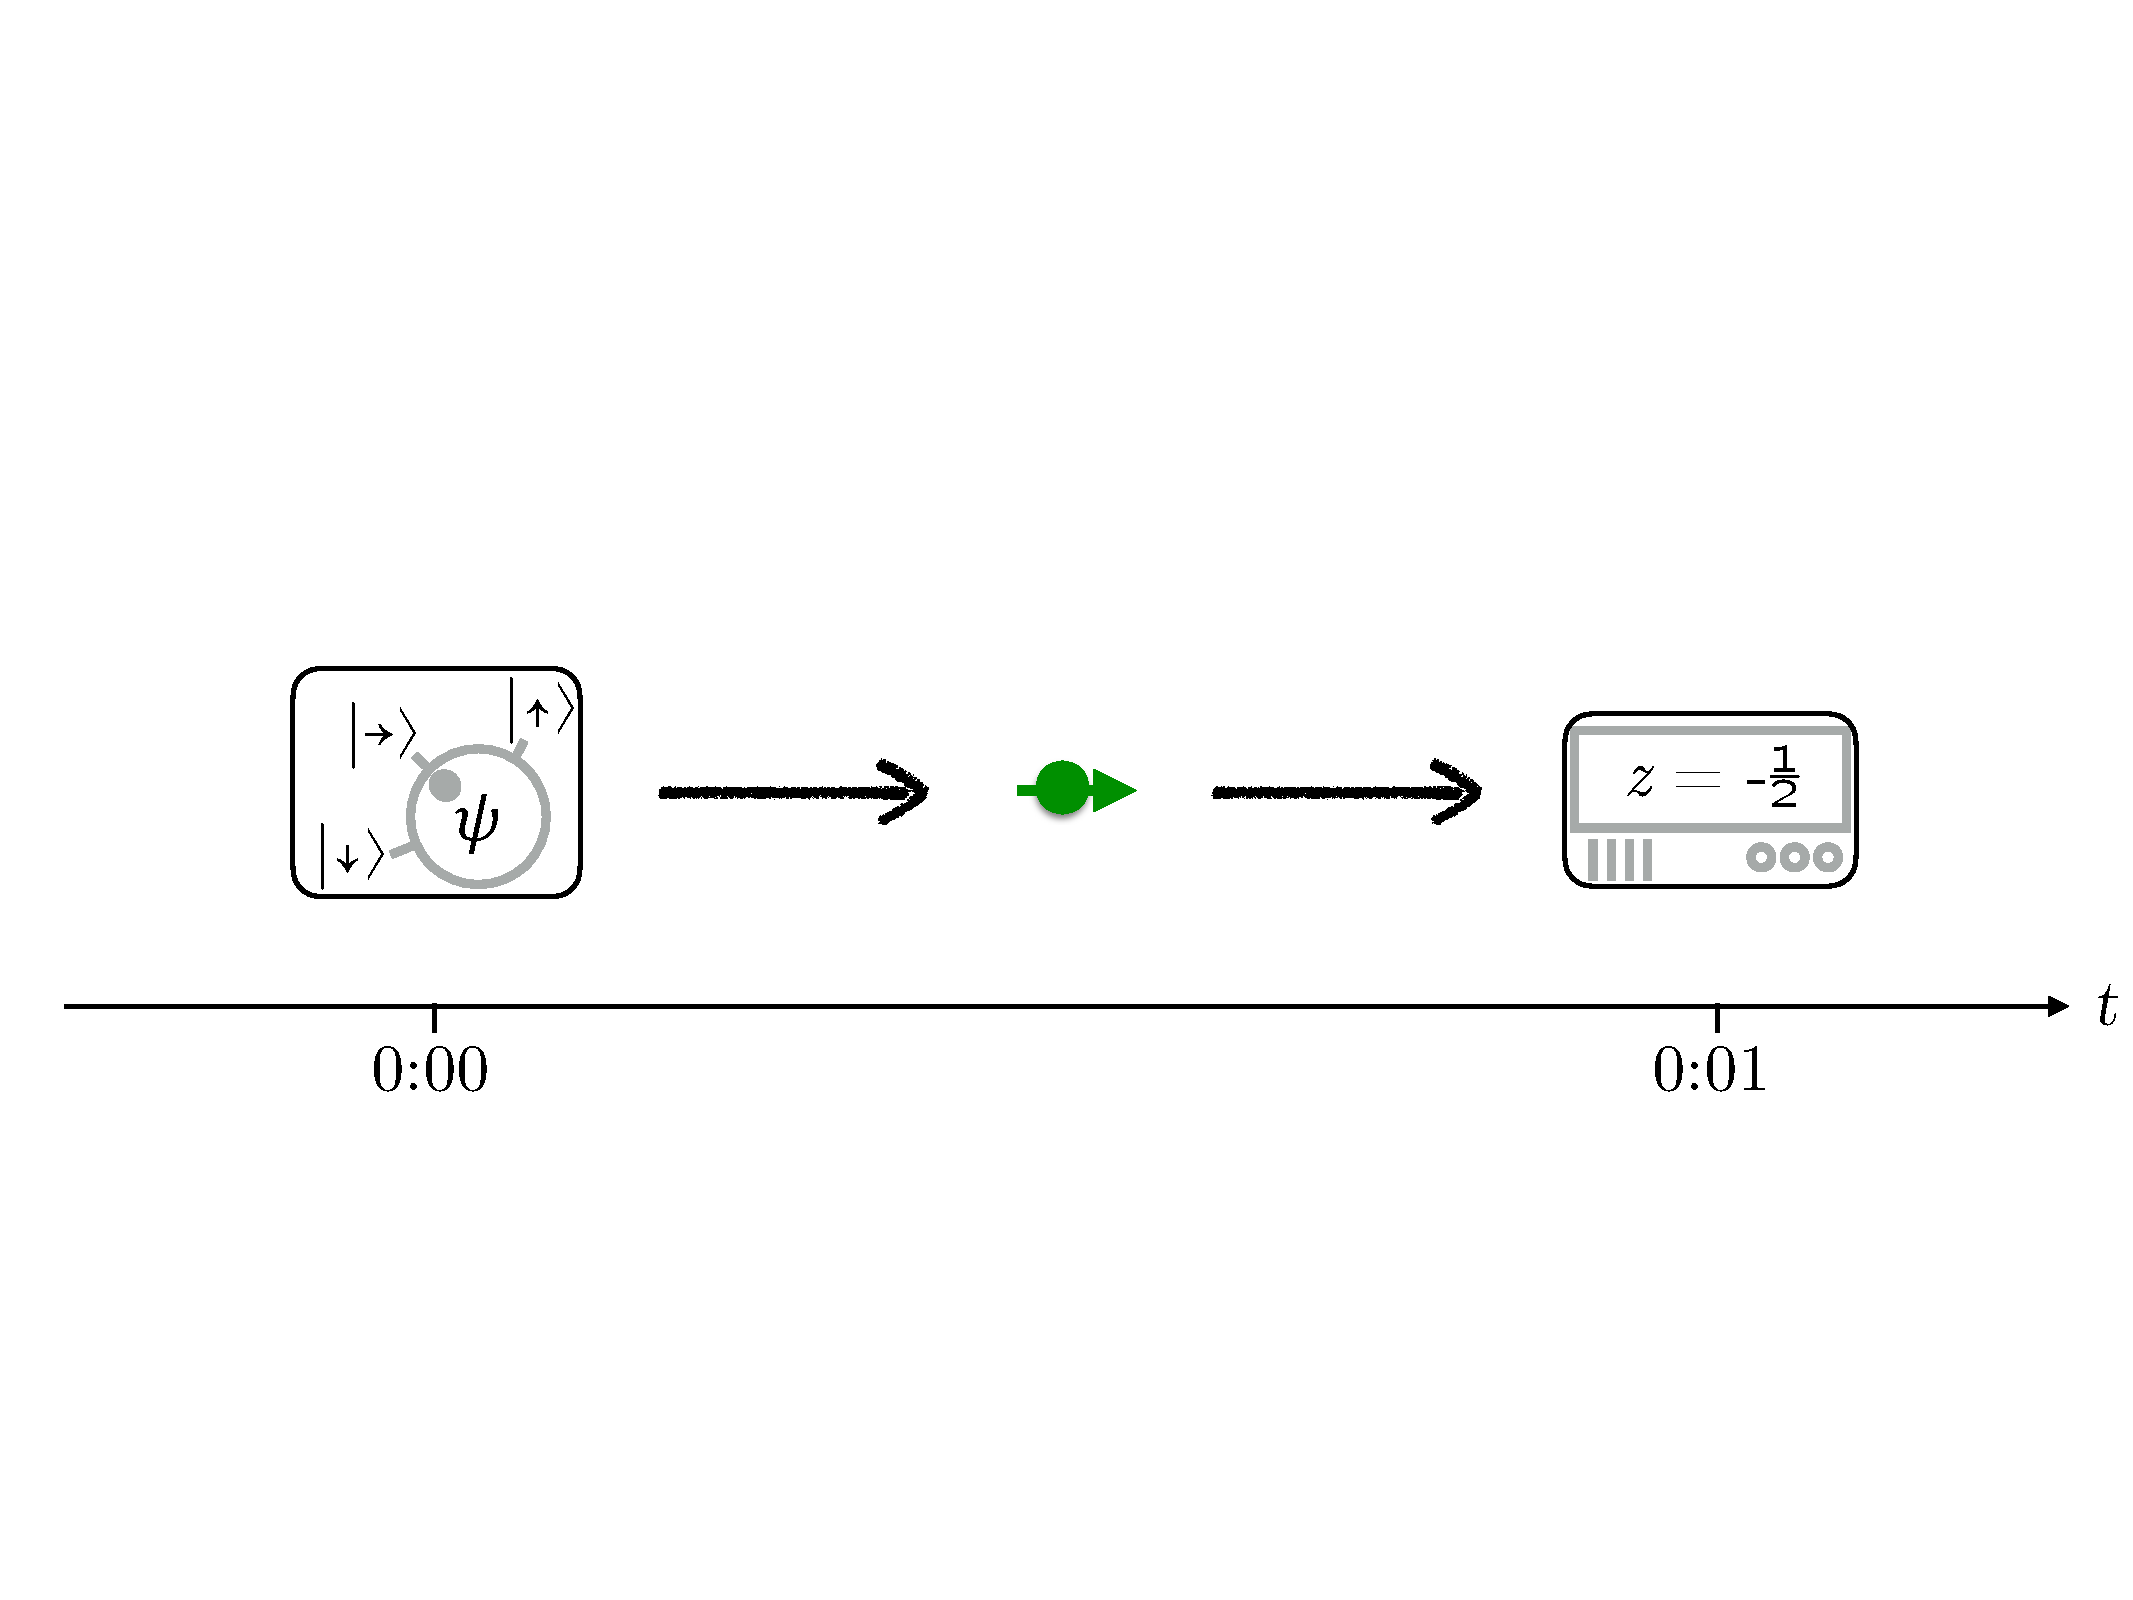
\includegraphics[trim= 0.4cm  8.6cm 0cm 11cm, clip=true, width=0.8\textwidth]{BasicMeasurement.pdf}
\caption{\emph{A basic quantum measurement experiment.} A  source emits an electron polarised according to $\psi$. The detector measures the vertical polarisation direction~$z$.
\label{fig_basicmeasurement}
}
\end{figure}

Physical theories that impose that quantum measurements have single outcomes are often called \emph{single-world interpretations}. (The term ``interpretation'' alludes to the fact that textbook quantum mechanics leaves open the question of how an expression such as~\eqref{eq_probstatement} should be translated to a statement such as~\eqref{SWClaim} or~\eqref{MWClaim}. It is hence necessary to interpret~\eqref{eq_probstatement}.)  The main contribution of this work is an argument which, adopting this terminology, asserts that single-world interpretations of standard quantum theory cannot be self-consistent.  More specifically, we prove a theorem that corresponds to the following informal claim. 

 \colorlet{shadecolor}{orange!15}
 \begin{shaded}
 \noindent \textbf{Main result (informal version)} \vspace{1ex}

 \noindent There cannot exist a physical theory $T$ that has all of the following properties: \vspace{-0.8ex}
  \begin{enumerate}[itemindent=0cm,labelsep=0.2cm,leftmargin=1.0cm] 
    \setlength{\itemsep}{0ex}
    \item[$\QT$]   \emph{Compliance with quantum theory:} $T$ forbids all measurement results that are forbidden by standard quantum theory (and this condition holds even if the measured system is large enough to contain itself an experimenter).
    \item[$\SW$]  \emph{Single-world:} $T$ rules out the occurrence of more than one single outcome if an experimenter measures a system once.
          \item[$\SelfCons$]  \emph{Self-consistency:} $T$'s statements about measurement outcomes are logically consistent (even if they are obtained by considering the perspectives of different experimenters).
              \end{enumerate} \vspace{-2ex}
 \end{shaded}
 
Property~$\QT$ refers to standard quantum theory, which does not impose any constraints on the complexity of objects it is applied to~\cite{Deutsch85}.  It is certainly legitimate to question whether a theory that accurately describes nature must respect this requirement | after all, we are still lacking experimental evidence for the validity of quantum theory on macroscopic scales.  Conversely, self-consistency, as defined by~$\SelfCons$, is arguably an unavoidable requirement to any reasonable physical theory.  We are thus left with two scenarios, depending on the outcome of future experiments. 
\begin{itemize}
  \item \emph{Scenario~1:} Experiments reveal that quantum theory is inaccurate in certain regimes and must be replaced by a different theory. (It could be, for instance, that we discover a yet unknown physical mechanism that leads to an ``objective collapse'' of the wave function.)
  \item \emph{Scenario~2:} Experiments confirm that quantum theory accurately describes systems as complex as experimenters who themselves apply quantum theory.  In this case, the result proved here forces us to reject a single-world description of physical reality. 
 \end{itemize}

A nice example that illustrates the use of the main result presented here is the \emph{de Broglie-Bohm theory}, also known as \emph{Bohmian mechanics} or \emph{pilot-wave theory}~\cite{deBroglie27,Bohm52,DuTe09}. According to this theory, measurement outcomes are determined by particle positions, which are well-defined at any time, so that~$\SW$ is satisfied. Bohmian mechanics is also compatible with quantum theory (without a ``collapse mechanism''), so that~$\QT$ holds, too. We must therefore conclude that it cannot satisfy~$\SelfCons$. That is, if Bohmian mechanics is applied from different experimenters' perspectives, one sometimes obtains mutually contradicting statements. In fact, the same conclusion holds more generally for any deterministic hidden variable theory. 

The paper is organised as follows.  In Section~\ref{sec_framework}, we introduce a (rather minimalistic) framework to formally capture the relevant aspects of different interpretations of quantum theory, such as single-world vs.\ many worlds. The main result is stated  in Section~\ref{sec_claim}. For its proof, we introduce in Section~\ref{sec_experiment} an extension of the Wigner's Friend gedankenexperiment~\cite{Wigner67}, which is then analysed in Section~\ref{sec_proof}. In Section~\ref{sec_discussion} we discuss specific theories that have been proposed, such as Bohmian mechanics, in the light of the results presented here. 


\section{Framework: Physics in terms of stories} \label{sec_framework}

\subsection{Physical theories as constraints on stories} \label{sec_phystheory}

The main result, as described informally in the introduction, refers to the notion of a \emph{physical theory}~$T$, and we should therefore spell out what we mean by this. Yet, all we need is a characterisation in terms of certain \emph{necessary} criteria. The reason is that the result asserts the \emph{non}-existence of a theory~$T$ with certain properties. Hence, the looser the definition we use for characterising $T$, the stronger is the claim (cf.\ Section~\ref{sec_theories}).
%\footnote{For example, the definition that we are going to use does not demand that a physical theory provides predictions for the outcomes of measurements in terms of probability distributions. This is in contrast to Bell's work, for instance, where probabilistic predictions are a indispensable part of the framework he uses.}

The approach we take is based on the paradigm that any physical theory~$T$ comes with a set of laws that ``forbid'' certain things from happening. For example, thermodynamics forbids  that heat flows from a cold to a hot body.  Another example would be a ``collapse theory'', which forbids that  a macroscopic object can be in a superposition of being at two distant locations.      This paradigm connects to the idea of  falsifiability. If an experiment leads to an observation that is forbidden by~$T$ then we have falsified $T$. Conversely, if nothing is forbidden by $T$ then $T$ cannot be experimentally falsified.

A basic ingredient to our approach is the notion of a \emph{story}, i.e., an account of events that occur. Specifically, we consider stories, real or fictitious, about experiments such as the spin measurement described in the introduction  (see Fig.~\ref{fig_basicmeasurement}). To expand on this example, suppose that the electron is emitted by a source that polarises it along a direction $\psi$ as indicated by the position of a knob. Right after, its vertical spin component is measured and the outcome $z$ is shown on the display of the measurement device.  In addition, there shall be a clock that shows time~$t$. A possible story may then read as follows. 
\begin{align*}
  s_1 = \textstory{At $t= \text{0:00}$ the source is invoked with knob position $\psi = \spinright$ and at $t= \text{0:01}$ the measurement device shows outcome $z = \sminus$.}
\end{align*}
Another story could be
\begin{align*}
  s_2 =  \textstory{At $t=\text{0:00}$ the source is invoked with knob position $\psi = \spinup$ and at $t= \text{0:01}$ the measurement device shows outcome $z =  \sminus$.}
\end{align*}
Many more stories are conceivable of course, and we will in the following denote by $\Sigma$ the set of all possible stories.  For our purposes, it is not necessary to characterise this set further | it suffices to simply postulate its existence.\footnote{In certain contexts it is useful to impose  that the set be countable, though.}  Yet, for concreteness, one may think of $\Sigma$ as the set of all finite sequences of letters or of all sequences of English words. Most of the stories then have no well-defined meaning, but this is unproblematic as we shall see later. 

Given a story $s \in \Sigma$, we may find that it contradicts certain laws of physics. In this sense, physical theories impose constraints on the set of all possible stories $\Sigma$ (Fig.~\ref{fig_theories}). For example, we would say that  quantum mechanics forbids story $s_2$, but not $s_1$.  This motivates the following characterisation of physical theories.
  
\begin{figure}[t]
\centering
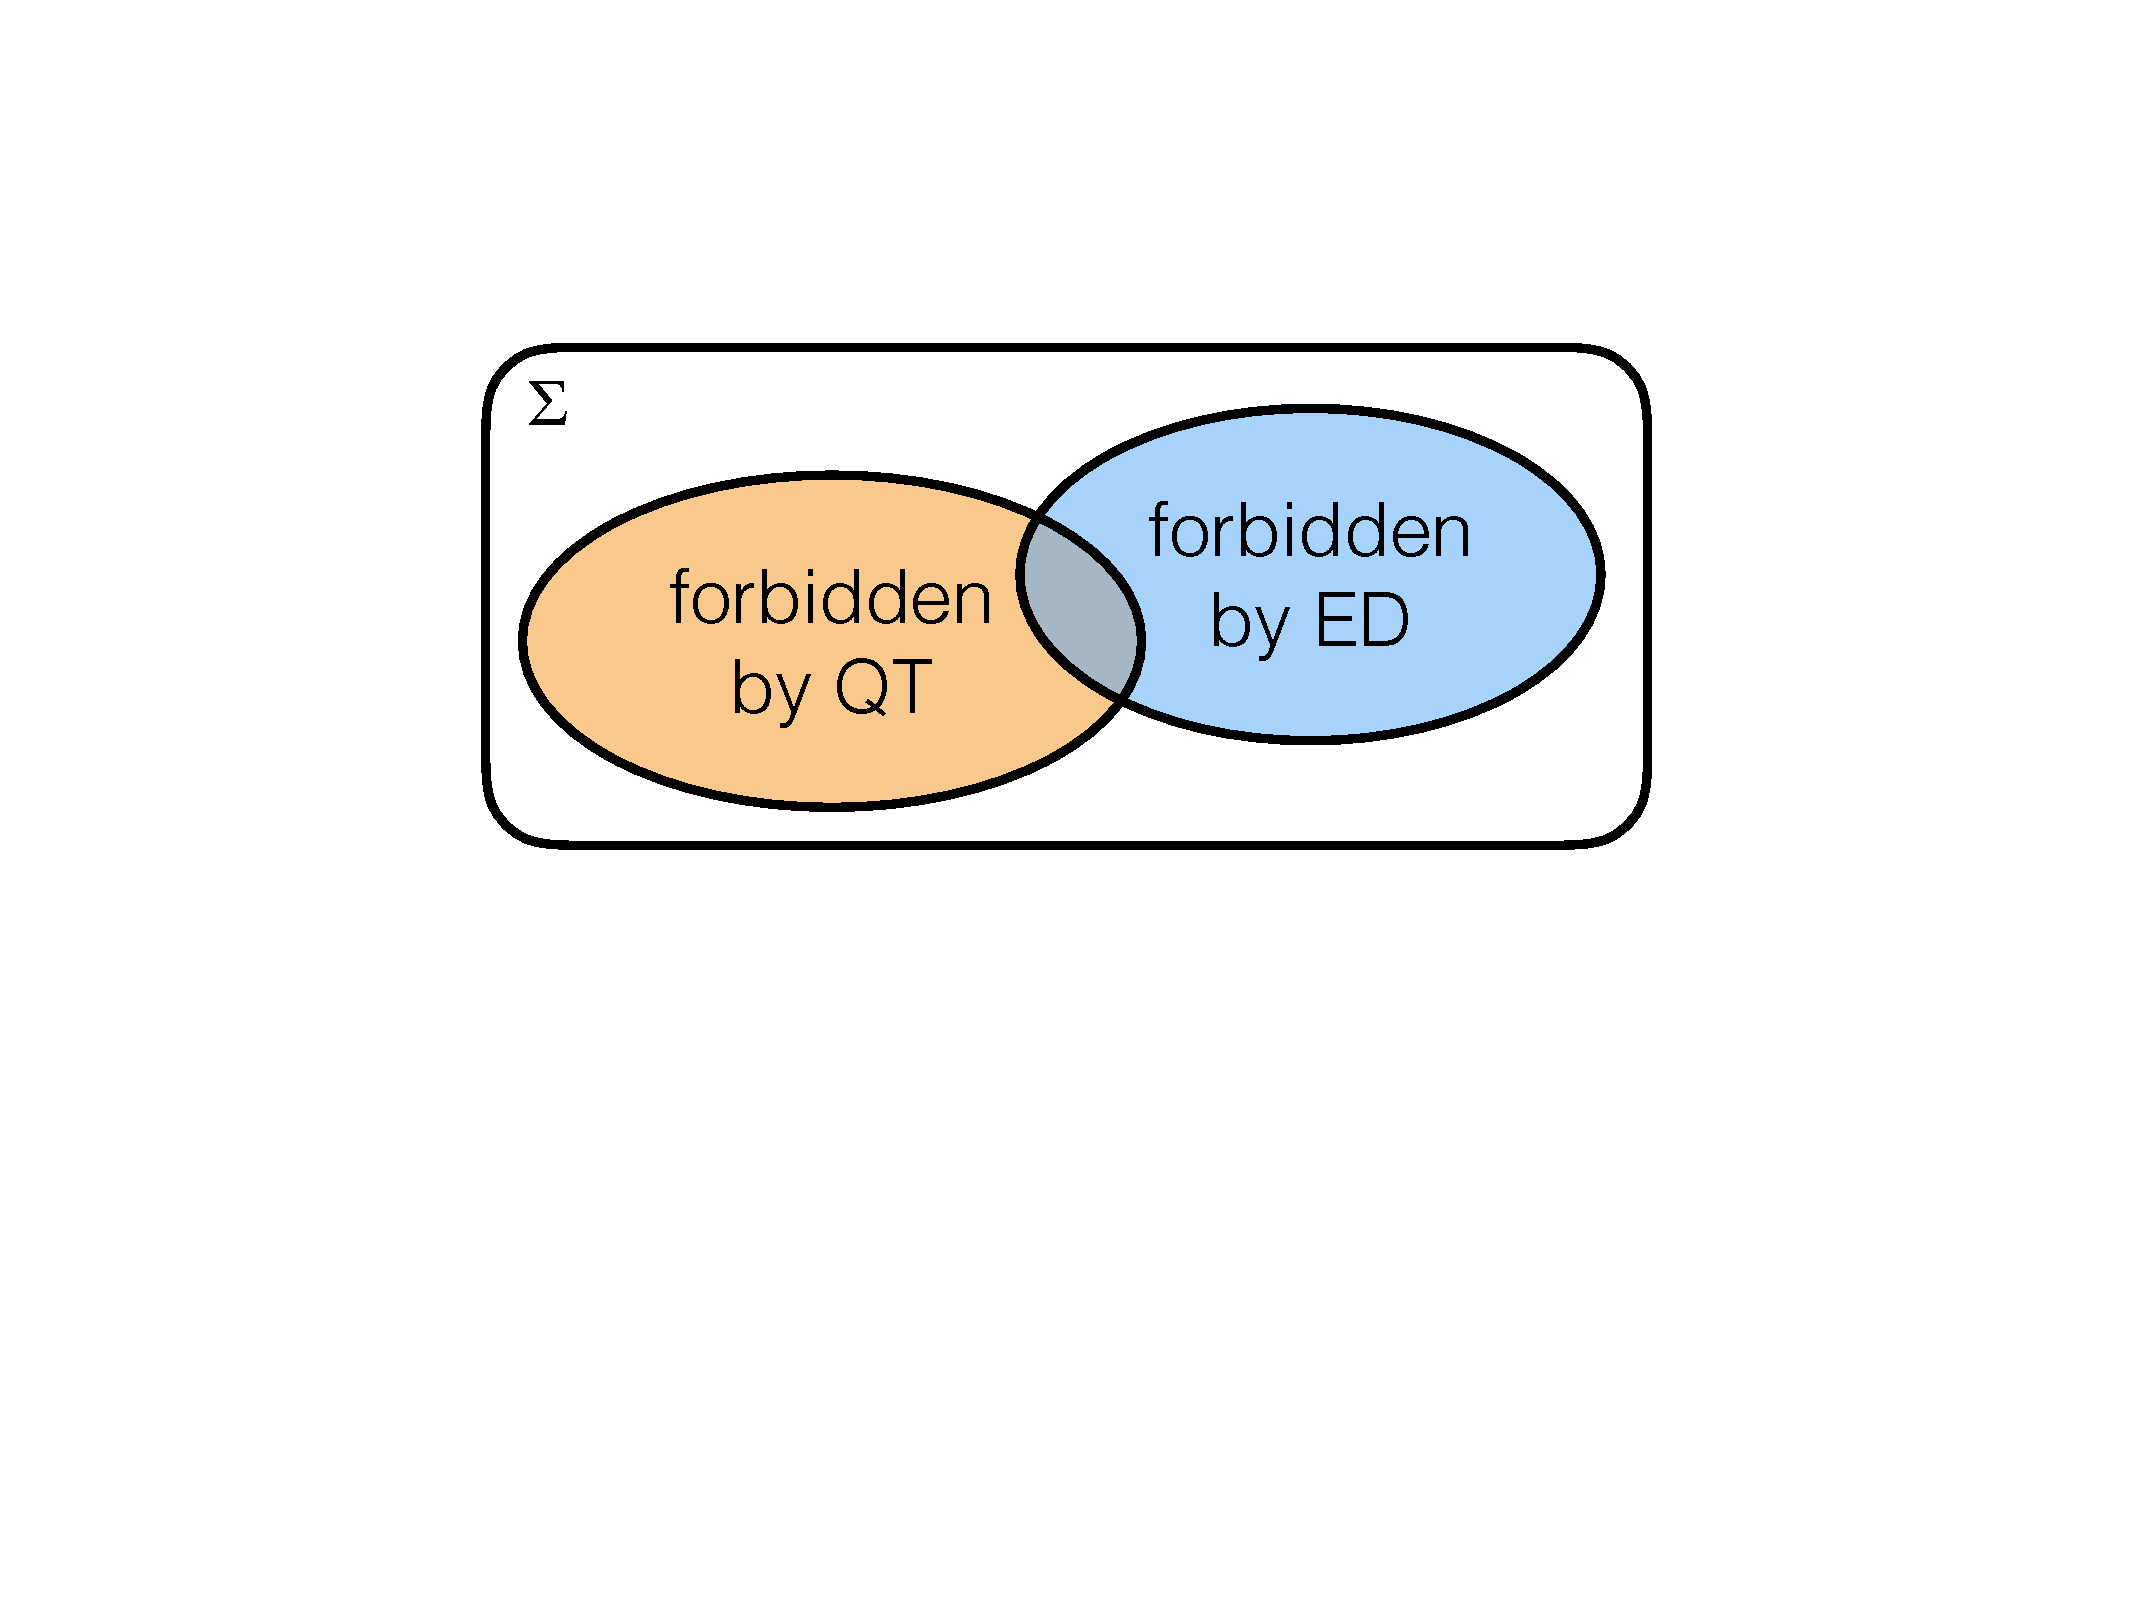
\includegraphics[trim= 0.4cm  12.5cm 0cm 5.5cm, clip=true, width=0.8\textwidth]{Theories.pdf}
\caption{\emph{Physical theories.}  $\Sigma$ is the set of all stories. Physical theories, such as quantum theory, QT, or electrodynamics, ED, rule out some of them. 
\label{fig_theories}
}
\end{figure}
  
 \colorlet{shadecolor}{orange!15}
 \begin{shaded}
 \noindent A \emph{physical theory}, $T$, specifies a subset of $\Sigma$, whose elements are called \emph{forbidden} stories. We write $s \notin T$ to indicate that $s \in \Sigma$ is forbidden by $T$.
\end{shaded}

The terminology is deliberately chosen in an asymmetric manner.   If a story $s \in \Sigma$ is not forbidden by a physical theory $T$, then this should not be interpreted as ``$s$ is allowed by $T$''.  For example, it could be that $s$ is not precise enough for $T$ to be applicable, or it could be that $s$  simply has no meaning. (Recall that we did not impose any constraints on the set of all stories $\Sigma$.)

\subsection{Interpreting stories in terms of their plots} \label{sec_plots}

A story, in the usual sense of the word, has a \emph{plot}, corresponding to the series of \emph{events} that happen according to it.  We will use this notion to specify, in a precise manner, what a story $s$ tells us about an experiment. To illustrate this, we may once again consider the spin measurement experiment of the introduction. This experiment has the following generic structure. 

\ExpBegin{Basic Measurement Experiment ($\BME$) }
  \noindent Given a quantum system with Hilbert space $\cH$ and a family of measurement projectors $\{\pi_z\}_{z \in \cZ}$ on $\cH$, perform the following steps at the corresponding times $t$.\footnotemark
 \vspace{1.4ex}

 \hspace{-0.6em}
\begin{tabular}{p{2.9em} p{0.82\textwidth}}
  @ 0:00 & Prepare the system in state $\psi$. \\
  @ 0:01 & Measure the system w.r.t.\  $\{\pi_z\}_{z \in \cZ}$ and record the outcome~$z$. \\
  @ 0:02 & Halt. 
\end{tabular}
\ExpEnd

 \footnotetext{Here and in the following, times indicated in an experiment should be understood as placeholders that can be substituted by any other points in time with the same order. Furthermore, we assume that the systems' states remain unchanged unless the protocol prescribes a specific action on them. In the present example, the evolution of the system's state between $t = \text{0:00}$ and $t = \text{0:01}$ shall hence be trivial. }

%We remark that, when describing experiments involving quantum systems, 
%The halting step is included to indicate that the experiment continues until $\text{0:02}$, in the sense that, for instance, a record of $z$ would be kept until then. 

When carrying out such an experiment, which we may call $\Exp$, we are typically interested in a well-defined set of events that may potentially occur. We denote this set by~$[\Exp]$. In the case of the spin measurement experiment, any  event of interest could, for instance, be identified with a particular reading of values shown by the clock, the source (whose knob position shows the prepared state), and the measurement device. This would motivate an event space of the form
\begin{align} \label{eq_BMEevents}
  [\Exp] = \bigl\{ (t, \psi, z) \in \cT \times \cH \times (\cZ \cup {\bot}) 
 % : \, z \neq \bot \text{  if } t = \text{0:01}
   \bigr\} \ ,
\end{align}
where  $\bot$ indicates that no outcome has been recorded, and where
\begin{align} \label{eq_timeset}
  \cT = \bigl\{\text{$n$:$m$}: \, n \in \mathbb{N}_0, \, m \in \{0, \ldots, 59\} \bigr\} 
\end{align}
is the set of possible time values~$t$ shown by the clock. This latter set is discrete, capturing the idea that the clock has a finite precision. 

Given the set $[\Exp]$ of \emph{potential} events that can happen in the experiment~$\Exp$, a story~$s$ about $\Exp$ now defines a \emph{plot} $s^{\Exp}$, i.e., a subset of events that \emph{actually} occur according to the story. For story~$s_1$ from Section~\ref{sec_phystheory}, for instance, the plot could be taken to be
\begin{align*}
% s_1^{\Exp} & = \bigl\{(t, \psi, z \in [\Exp] : \, \psi = \begin{cases} \spinright & \text{ if $t < \text{0:01}$} \\ \mathbf{0} & \text{otherwise} \end{cases} \\ 
 s_1^{\Exp} & =  \bigl\{ (\text{0:00}, \spinright, \bot),  (\text{0:01}, \mathbf{0},  \sminus) \bigr\} \ .
 \end{align*}
 (The assignment $\psi = \mathbf{0}$ shall indicate that the measurement is interpreted as a destructive one.)  Similarly, for $s_2$, a natural choice could be
 \begin{align*}
  s_2^{\Exp} & = \bigl\{ (\text{0:00}, \spinup, \bot),  (\text{0:01}, \mathbf{0},  \sminus) \bigr\} \ .
\end{align*}
The plots $s_1^{\Exp}$ and $s_2^{\Exp}$ thus correspond to interpretations of the stories $s_1$ and $s_2$, which were described in prose, declaring precisely which events ``happen'' according to them. This idea is captured more generally by the following definition.

\begin{shaded}
  \noindent An \emph{experiment}, $\Exp$, specifies a set of \emph{events}, denoted by $[\Exp]$, as well as a function that assigns to certain stories $s \in \Sigma$ a subset $s^\Exp$ of $[\Exp]$,  called \emph{plot} of $s$. 
\end{shaded}

We note that, formally, there is no constraint on how a story $s$ is being interpreted in terms of a plot $s^\Exp$ | in principle $s^\Exp$ can be chosen arbitrarily. For our purposes, it will only be relevant that the interpretations of a story in different experiments are compatible with each other, in a sense that we are going to describe in Section~\ref{sec_views} below. 

In general, a story $s$ could be ambiguous about whether or not a certain event in $[\Exp]$ occurs. It could also be that $s$ does not talk about the experiment $\Exp$ at all.  In such cases one may of course not want to assign a plot $s^{\Exp}$ to $s$. The above definition accounts for this, as it does not demand that  $s^{\Exp}$ exists for all $s \in \Sigma$.  In other words,  $s \mapsto s^{\Exp}$ is generally a \emph{partial} function on $\Sigma$.

Importantly, the notion of a plot allows us to formally capture  different interpretations of quantum theory.  While, for instance, the stories $s_1$ and $s_2$ above are in agreement with a single-world interpretation, one could also consider other stories, according to which the measurement provokes a branching, with different outcomes being observed in the different branches. For example, we may define a story $\tilde{s}_1$ with plot
\begin{align*}
  \tilde{s}_1^{\Exp} & =  \bigl\{ (\text{0:00}, \spinright, \bot),  (\text{0:01}, \mathbf{0},  \sminus), (\text{0:01}, \mathbf{0},  \splus)  \bigr\} \ ,
\end{align*}
i.e., both outcomes $z = \sminus$ and $z = \splus$ occur according to this story. 


\subsection{Different views on the same story} \label{sec_views}

Two experimenters may have different views on the same experimental setup and therefore describe it in two different ways. Consequently, their interpretation of a given story $s$ in terms of its plot will in general also be different. Nevertheless, the two plots must of course still be compatible. 

%, in a sense that we are going to describe now.  But first a note on notation: In situations where this is unambiguous, we  denote by~$\Exp$ the experiment as viewed by experimenter~$\Exp$, and likewise $\Expp$ for the experiment as viewed by~$\Expp$. 

To explain what we mean by this, we first  consider a simple situation where an experiment~$\Exp$, as viewed by one experimenter,  is a part of a larger experiment~$\Expp$, as viewed by another experimenter. An example of such a larger experiment could be an  extension of the spin measurement experiment from above where, in addition to the measurement at time $t = \text{0:01}$, a second spin measurement with outcome $z'$ is carried out at $t = \text{0:02}$.  The event space $[\Expp]$ of~$\Expp$ may therefore be defined as the set of  quadruples $(t, \psi, z, z')$. However, when describing~$\Exp$ we may ignore the second measurement, so that $[\Exp]$ consists of triples $(t, \psi, z)$. 

Formally,  the two experiments are defined by (partial) functions~$s \mapsto s^{\Exp}$ and  $s \mapsto s^{\Expp}$ from the set of stories $\Sigma$ to $[\Exp]$ and $[\Expp]$, respectively.  The functions specify how a given story $s$ should be interpreted. While the plots $s^{\Exp}$ and $s^{\Expp}$ may in principle be defined arbitrarily, we want to model that $\Exp$ is a part of $\Expp$. This is done by imposing certain \emph{compatibility constraints}. For instance, we may demand that any event $(t, \psi, z, z')$ that occurs in experiment~$\Expp$ must correspond to an event $(t, \psi, z)$ that occurs in the part~$\Exp$. This could be captured by the compatibility constraint
\begin{align*}  
  (t, \psi, z) \in s^{\Exp} \quad \iff \quad \exists \, z' : \, (t, \psi, z, z') \in s^{\Expp}  \ ,
\end{align*} 
which should hold for any story~$s$ for which $s^{\Expp}$ is defined.  To simplify the notation, we will in the following abbreviate terms of the form $\exists \, y : \, (x, y)$ by $(x, *)$. The compatibility constraint can then be rewritten as 
\begin{align} \label{eq_subexperiment}
  (t, \psi, z) \in s^{\Exp} \quad \iff \quad (t, \psi, z, *) \in s^{\Expp}  \ .
\end{align} 

More generally, two experiments, $\Expone$ and $\Exptwo$, may just have an overlap, but not be contained in each other. Suppose for example that both of them include a measurement of  time $t$ as well as some quantity~$z$, but in addition also separate quantities, $z_1$ and $z_2$, so that their event spaces, $[\Expone]$ and $[\Exptwo]$, consist of triples $(t, z, z_1)$ and $(t, z, z_2)$, respectively.  The compatibility constraint that models that the two experiments have the quantities $t$ and $z$ in common could then be formulated as the condition that
\begin{align} \label{eq_overlapexperiment}
  (t, z, *) \in s^{\Expone} \quad \iff \quad (t, z, *) \in s^{\Exptwo} 
\end{align} 
holds for any story~$s$ for which both $s^{\Expone}$ and~$s^{\Exptwo}$ are defined. 

We stress that, in the logic of the framework, compatibility constraints such as~\eqref{eq_subexperiment} and~\eqref{eq_overlapexperiment} are not derived relations, but rather \emph{define} how the different experiments are related. In other words, \eqref{eq_subexperiment} defines what we mean when we say that experiment~$\Exp$ is a part of experiment~$\Expp$. Similarly, \eqref{eq_overlapexperiment} defines what we mean when we say that $\Expone$ and $\Exptwo$ have the quantities~$t$ and~$z$ in common. 



\subsection{Representation of physical laws}

Recall that physical laws correspond to rules that forbid certain stories.  To formulate these rules, it is often convenient to consider  specific experiments. The rules then take the form of conditions on the plots of the stories, which can be expressed in mathematically precise terms.  

To illustrate this, consider the quantum-mechanical law that the measurement of a quantum system with respect to projectors $\{\pi_{z}\}_{z \in \cZ}$ will with certainty give outcome $\hat{z}$ if the prepared state $\psi$ satisfies $\|\pi_{\hat{z}} \psi \| = 1$.  To formalise this law, let  $\BME_{\cH, \{\pi_z\}}$ be the set of all experiments $\Exp$ that have the form of the Basic Measurement Experiment introduced in Section~\ref{sec_plots}. Formally, their event space $[\Exp]$ is defined by~\eqref{eq_BMEevents}, and the introductory spin measurement example would correspond to the case where $\cH = \mathrm{span}\{\spinup, \spindown\}$ and  where $\pi_{\frac{1}{2}}$ and $\pi_{-\frac{1}{2}}$ are projectors along $\spinup$ and $\spindown$, respectively. The law that $\hat{z}$ occurs if $\|\pi_{\hat{z}} \psi \| = 1$ can then be written as 
\begin{align} \label{eq_certainoutcome}
   (\text{0:00}, \psi, *) \in s^{\Exp}  \text{ and } \|\pi_{\hat{z}} \psi \| = 1 \quad \implies \quad   (\text{0:01}, *, \hat{z}) \in s^{\Exp} \ .
\end{align}
That a theory~$T$ contains this law now means that the implication
\begin{align} \label{eq_basicQM}
  \text{\eqref{eq_certainoutcome} is violated for some $\Exp \in \BME_{\cH, \{\pi_z\}}$}  \quad \implies \quad s \notin T
  \end{align}
  holds for any story~$s$. Applying this criterion to the above examples, we find that $s_2$ is forbidden, whereas $s_1$ and $\tilde{s}_1$ are not.  

The rule~\eqref{eq_basicQM} manifestly depends on the set of experiments $\BME_{\cH, \{\pi_z\}}$. This set therefore \emph{defines} the range of applicability of the corresponding physical law. It can in principle be chosen arbitrarily.  For example, if one holds the position that quantum mechanics is only valid  on microscopic scales, one may restrict $\BME_{\cH, \{\pi_z\}}$ to experiments where the measured system is small in some sense. Conversely, if one assumes that quantum theory extends to macroscopic systems then the set should also include, for instance, arbitrary quantum measurements on cats~\cite{Schroedinger35}.

In Section~\ref{sec_claim} we will use a generalisation of~\eqref{eq_basicQM} to express formally what we mean when we say that a theory $T$ complies with quantum theory.  The generalisation will include experiments where the system's state evolves non-trivially and where the measurement may be repeated.


\section{Main result} \label{sec_claim}

The main result, which will be stated as Theorem~\ref{thm_main} below, refers to three properties that a physical theory may, or may not, have.  In the following we describe them using the story-based approach introduced in Section~\ref{sec_framework}. 

\subsection{Compliance with quantum theory~$\QT$} \label{sec_QT}

Property~$\QT$ corresponds to the assumption that the laws of standard quantum theory are valid.  In fact, for our purposes, it suffices to restrict to some particular rules that are implied by standard quantum theory, i.e., we do not need to provide a full characterisation of  the theory.  To specify these rules, we consider the following experiment.

\ExpBegin{Repeated  Measurement Experiment ($\RME$)}
\noindent  Given a quantum system with Hilbert space $\cH$, a unitary $U$ on~$\cH$, a family of measurement projectors $\{\pi_z\}_{z \in \cZ}$ on $\cH$, and a value $\hat{z} \in \cZ$, repeat the following steps for increasing $n \in \mathbb{N}_0$ until the halting criterion is  satisfied.
 \vspace{1.4ex}
 
 \hspace{-0.6em}
\begin{tabular}{p{2.9em} p{0.82\textwidth}}
  @ $n$:00 & Prepare a quantum system in state $\psi$. \\
   & Let the system evolve according to~$U$. \\
  @ $n$:01 & Measure the system w.r.t.\ $\{\pi_z\}_{z \in \cZ}$ and record the outcome~$z$. \\
  @ $n$:02 & Halt if $z =\hat{z}$.\footnotemark 
\end{tabular}
\ExpEnd
\footnotetext{The halting step is not strictly needed. But since we are mostly interested in the case where $\pi_{\hat{z}} \psi \neq 0$, and since $\QT$ then implies that the experiment will end after finite time, it avoids the need for stories that talk about an infinite sequence of measurements.}
To simplify the notation, we will in the following represent the measurement projectors $\{\pi^H_z\}_{z \in \cZ}$ in the Heisenberg picture, i.e., 
\begin{align}
  \pi^H_z = U^{\dagger} \pi_z U \ .
\end{align}

While standard quantum theory generally makes probabilistic predictions, it also implies certain deterministic statements. In particular, the following must hold for any fixed $\hat{z} \in \cZ$.
\begin{enumerate}[label=(\emph{\alph*})]
  \item If the prepared state $\psi$ satisfies $\|\pi^H_{\hat{z}} \psi\| = 0$ in round $n$ then the outcome $z = \hat{z}$ does not occur in this round.
    \item If the prepared state $\psi$ satisfies $\|\pi^H_{\hat{z}} \psi\| = 1$ in round $n$ then the outcome $z = \hat{z}$ occurs in this round.
  \item If the prepared state $\psi$ satisfies $\|\pi^H_{\hat{z}} \psi \| \neq 0$ and is identical in all rounds~$n$ until the halting criterion is satisfied then the outcome $z = \hat{z}$ occurs at some point.
  \end{enumerate}
The definition of~$\QT$ below captures the idea that any theory $T$ that complies with quantum theory must satisfy these rules. 

To formalise the rules within our framework, let $\RME_{\cH, \{\pi^H_z\}}$ be the set of all experiments of the type above, for any given Hilbert space $\cH$ and a family of measurement projectors $\{\pi^H_z\}_{z \in \cZ}$ in the Heisenberg picture. On the formal level, we demand that the event space of any $\Exp \in \RME_{\cH, \{\pi^H_z\}}$ is of the form (see also~\eqref{eq_BMEevents})
\begin{align*} 
    [\Exp] = \bigl\{ (t, \psi, z) \in \cT \times \cH \times (\cZ \cup {\bot})      \bigr\}  \ ,
    % : \, z \neq \bot \text{  if } t = \text{$n$:01} \text{ for } n \in \mathbb{N}_0 
\end{align*}
where $\cT$ is defined by~\eqref{eq_timeset}. The set $\RME_{\cH, \{\pi^H_z\}}$  may otherwise be chosen arbitrarily, provided that it includes the relevant parts of the Extended Wigner's Friend Experiment defined in Section~\ref{sec_experiment} below. This requirement will be captured formally by the conditions~\eqref{eq_FriendoneM}, \eqref{eq_FriendtwoM}, \eqref{eq_AssistantM}, and~\eqref{eq_WignerM}. 

The properties of a story~$s$ that are relevant for the formulation of~$\QT$ can be written as conditions on the plots $s^{\Exp}$ for $\Exp \in \RME_{\cH, \{\pi^H_z\}}$. For example,  that the experiment is repeated until the halting condition is satisfied corresponds to the implication
\begin{multline} \label{eq_untilhalt}
  n=0 \text{ or } (\text{$(n-1)$:01}, *, z) \in s^{\Exp} \text{ for $z \neq \hat{z}$} \\
  \quad \implies \quad \forall \, t \in [\text{$n$:00}, \text{$n$:01}] :\, (t, *, *) \in s^{\Exp} \ .
\end{multline}
For convenience, we also define the set  
\begin{align*}
  \Psi_n(s) = \{ \psi : \, (\text{$n$:00}, \psi, *) \in s^{\Exp} \} \ ,
\end{align*}
telling us which states are prepared in round~$n$ according to story~$s$. (If $s$ talks about many worlds, for instance, this set could contain more than one element.)

\begin{shaded}
  \noindent \emph{$T$ satisfies $\QT$} means that~$T$ forbids all stories $s$ according to which in some experiment $\Exp \in \RME_{\cH, \{\pi^H_z\}_z}$ and for some $\hat{z} \in \cZ$ one of the following happens. \nobreak
      \begin{enumerate}[label=(\emph{\alph*}),itemindent=0cm,labelsep=0.4em,leftmargin=1.7em]
     \item  In some  round $n$, any $\psi \in \Psi_n(s)$ satisfies $\|\pi^H_{\hat{z}} \psi\| = 0$. Yet $(\text{$n$:01}, *, \hat{z}) \in s^{\Exp}$ holds.  \label{it_QMa}
     \item In some round $n$, some $\psi \in \Psi_n(s)$  satisfies $\|\pi^H_{\hat{z}} \psi\| = 1$. Yet $(\text{$n$:01}, *, \hat{z}) \in s^{\Exp}$ does not hold.  \label{it_QMb}
      \item The experiment is repeated, i.e., \eqref{eq_untilhalt} is satisfied, with $\Psi_n(s) = \{\psi\}$ for $\psi$ fixed such that  $\|\psi^H_{\hat{z}} \psi\| \neq 0$.  Yet $(\text{$n$:01}, *, \hat{z}) \in s^{\Exp}$ holds in no round $n$. \label{it_QMc}
           \end{enumerate}
    \vspace{-1.7ex}
    \end{shaded}
    
 Note that, according to standard quantum theory, all these conditions hold with certainty. 
   
% These criteria are  rather weak. They do not imply, for instance, that the theory $T$ predicts the same statistics of the measurement outcomes as quantum theory. But, as discussed earlier, this is fine, as we only need a necessary criterion for when a theory $T$ should be considered compatible with quantum theory. 

\subsection{Single-world~$\SW$}

Property~$\SW$ captures the idea that a measurement on a quantum system has only one single outcome. More specifically, we demand that this is the case for all quantum measurements relevant to one particular experimenter. (In the language of~\cite{Brukner15}, this could be regarded as the requirement that there are ``facts'' | maybe not ``per se'', but at least ``relative to an observer''.) 

To formalise this property, let $\BOE$ be a set of experiments of the form of the Repeated Measurement Experiment as defined in Section~\ref{sec_plots}. That is, any $\Exp \in \BOE$ is also an element of $\RME_{\cH, \{\pi^H_z\}}$, where $\cH$  is a Hilbert space and $\{\pi^H_z\}_{z \in \cZ}$ a family of projectors. Crucially, the set $\BOE$ may be restricted to those experiments that describe the viewpoint of one single experimenter. In the Extended Wigner's Friend Experiment, this will be Wigner, i.e., we will demand that the experiment $\Wigner$, defined in Section~\ref{sec_expview}, is included in this set (cf.\ \eqref{eq_WignerM} below). 

\begin{shaded}
  \noindent  \emph{$T$ satisfies $\SW$} means that~$T$ forbids all stories $s$ according to which for some experiment $\Exp \in \BOE$ the set
  \begin{align*}
    \bigl\{ z \in \cZ: \,  (\text{0:01}, *, z) \in s^{\Exp}\bigr\}
   \end{align*}    
   has more than one single element.
\end{shaded}



We remark that $\SW$ is fundamentally different from the requirement that a theory $T$ be deterministic. For example, $T$ may prescribe that the outcome of a spin measurement is either $z = \sminus$ or $z = \splus$ (not both), but still assert that this outcome is not correlated to anything that can be known before the measurement is carried out. 

%As before, this condition applies to any story $s$ that talks about an experiment which contains $\BOE$ as a part. Examples are the stories $s_1$, $s_2$, and $\tilde{s}_2$ about the Basic Measurement Experiment as defined in Section~\ref{sec_framework}.

\subsection{Self-consistency $\SelfCons$}

Property~$\SelfCons$ is the requirement of self-consistency. Generally speaking, it demands that the laws of a theory~$T$ do not contradict each other. To express this formally,  let $\allExp$ be the set of all experiments that the theory should be able to talk about. For us, it is sufficient to demand that $\allExp$ includes the experiments $\Friendone$, $\Friendtwo$, $\Assistant$, and $\Wigner$, as defined in Section~\ref{sec_experiment} below. 

%For example, if a theory has a law which asserts that the outcome of a measurement is an odd number, whereas another law of the theory implies that it must be even, thus excluding any possible outcome, we would say that the theory is not self-consistent. 



%\begin{shaded}
%  \noindent When we say that a \emph{physical theory $T$ satisfies $\SelfCons$} then this means that the condition  
%  \begin{align*}
%     \forall \Exp \in \BOE \, \forall t \in [\text{0:01}, \text{0:02}) : \,  (t, *) \in s^{\Exp}
%  \end{align*}
%  should not imply that $s$ is forbidden by $T$. 
%\end{shaded}
%
%\RR{This may be further simplified to the following condition.}

\begin{shaded}
  \noindent \emph{$T$ satisfies $\SelfCons$} means that the condition  
  \begin{align*}
      s^{\Exp} \text{ is defined for all }   \Exp \in \allExp 
  \end{align*}
  does not imply that $s$ is forbidden by $T$. 
\end{shaded}

%We recall that, as for the previous properties, this should be interpreted as a necessary (but not sufficient) criteria for when a theory $T$ should be considered self-consistent. 

To illustrate this, let $\Expone$ and $\Exptwo$ be the two experiments described in Section~\ref{sec_views}. Suppose that a theory~$T$ forbids any story $s$ according to which $z_1 = \sminus$ in experiment~$\Expone$, as well as any story according to which $z_2 = \splus$ in experiment~$\Exptwo$. If, in addition, $T$ requires that $z = z_1$ holds in~$\Expone$ and that $z = z_2$ holds in $\Exptwo$ then there is obviously no story $s$ left that satisfies all rules of the theory.  Hence, assuming that $\Exp, \Expp \in \allExp$, the theory~$T$ violates the self-consistency condition $\SelfCons$, i.e., it rules out any possible story about the two experiments.




%To illustrate this, suppose that a theory $T$ has two laws, denoted by (L$_{k}$) for $k=1, 2$. These shall be defined by the rule 
%\begin{align*}
%   \exists (t, z, z_k) \in s^{\Exp_i} : \, z = 2 z_k + k \quad \implies \quad s \notin T \ , 
%\end{align*}
%where $\Exp_k$ is an experiment with event space $[\Exp_k]  = \{(t, z, z_k) \in \mathbb{R} \times \mathbb{Z} \times \mathbb{Z} \}$. Furthermore, the compatibility constraint $(t, z, z_k) \in s^{\Exp_k}  \iff (t, z) \in s^{\Exp}$ should hold for some $\Exp \in \cE$. Finally, the experiment should be such that at, say, time $t = \text{0:01}$, some value $z$ is observed, i.e., 
%\begin{align} \label{eq_someobservation}
%   (\text{0:01}, *) \in s^{\Exp_k}  
%\end{align}
%should hold for all $s$ for which a plot $s^{\Exp}$ is defined. 
%
%The law~(L$_1$) obviously forbids all stories $s$ where $z$ is an odd number, whereas (L$_2$) forbids all stories where $z$ is an even number. But this implies that, for all stories $s$ that are not forbidden by $T$, condition~\eqref{eq_someobservation} is violated, so that $s^{\Exp}$ is undefined.   Hence, $T$ does not satisfy~$\SelfCons$.


\subsection{Theorem}

We are now ready to state the main claim. 

\begin{shaded}
\begin{theorem} \label{thm_main}
  No physical theory $T$ can satisfy $\QT$, $\SW$, and $\SelfCons$. 
\end{theorem}
\end{shaded}


\section{Extended Wigner's Friend Experiment} \label{sec_experiment}

The proof of Theorem~\ref{thm_main} is based on an extension of the Wigner's Friend gedan\-ken\-ex\-peri\-ment~\cite{Wigner67}, which is similar to the Schr\"odinger's cat experiment~\cite{Schroedinger35}. Wigner considered an experimenter, the \emph{friend}, who carries out a measurement while being enclosed in a perfectly isolated lab. The time evolution of the experimenter's state (including the lab) then corresponds to that of a closed system. The extension is inspired by Deutsch's idea of ``undoing'' this measurement and verify whether the original state can be retrieved~\cite{Deutsch85}. The specific setup considered here is similar to one proposed recently by Brukner, which involves multiple experimenters who carry out a Bell test~\cite{Brukner15}.\footnote{As discussed at the end of Section~\ref{sec_vSW}, the argument presented here leads to different conclusions, though.}  As a  core ingredient we use a construction that originates in work by Hardy, where it was used to establish Bell's theorem without inequalities~\cite{Hardy92,Hardy93}.\footnote{Specifically, the global state~\eqref{eq_global} between $\Friendone$ and $\Friendtwo$ corresponds to Eq.~1 of~\cite{Hardy93} for the case where $\alpha^2 =  (3 + \sqrt{5})/6$.}  

We note that the purpose of the experiment is to prove Theorem~\ref{thm_main}. We therefore do not have to worry about its technological feasibility at this point. We only need to ensure that none of the steps of the experiment are forbidden by the basic laws of physics. The experiment has hence a similar status as, for instance, the Schr\"odinger's cat gedankenexperiment. Nevertheless, a reader being worried about experimenters (or cats) enclosed in perfectly isolated labs may substitute them by quantum computers which simulate their actions. 

In Section~\ref{sec_birdseye} we first describe the Extended Wigner's Friend Experiment informally.  We will do this in terms of an experimental protocol that prescribes the actions of the different participating experimenters from an overall perspective. Then, in Section~\ref{sec_expview}, we provide a  formal characterisation using the story-based framework introduced in Section~\ref{sec_framework}. For this, we specify the views of the different experimenters individually. 

\subsection{A bird's eye view on the experiment} \label{sec_birdseye} 

The Extended Wigner's Friend Experiment features four experimenters  (see Fig.~\ref{fig_EWF}). Two of them, the friends $\Friendone$ and $\Friendtwo$, shall be located in  separate labs. We assume that, from an outside perspective, they can be treated as isolated quantum systems | unless there are explicit communication steps in the experimental protocol. This means that the time evolution of their state is described by a unitary.  We also assume that $\Friendone$ is fully informed about the state of $\Friendtwo$ (including $\Friendtwo$'s entire lab) at the time when the experiment starts, and that this state is therefore pure. The other two experimenters, Wigner $\Wigner$ and his assistant $\Assistant$, are not only informed about the initial states of $\Friendone$ and $\Friendtwo$, but can also carry out arbitrary quantum measurements on them.

\ExpBegin{Extended Wigner's Friend Experiment ($\EWFE$)} 
\noindent Repeat the following steps for increasing $n \in \mathbb{N}_0$ until the halting criterion in the last step is satisfied. 

\vspace{1.4ex}

 \hspace{0.2em}
\begin{tabular}{p{2.9em} p{0.82\textwidth}}
@ $n$:00 & $\Friendone$ invokes a quantum random number generator and memorises the output $r \in \{\head,\tail\}$. \\[1ex]
@ $n$:10& Depending on whether $r=\head$ or $r=\tail$, $\Friendone$ sets the spin~$\Spin$ of an electron to state $\spindown_\Spin$ or~$\spinright_\Spin$,  respectively, and hands it over to $\Friendtwo$. \\[1ex]
@ $n$:20 & $\Friendtwo$ measures $\Spin$ with respect to the basis $\{\spindown_\Spin, \spinup_\Spin\}$ and memorises the outcome $z \in \{\sminus, \splus\}$.  \\[1ex]
@ $n$:30 &  $\Assistant$ measures $\Friendone$ with respect to a basis $\{\ket{\ok}_{\Friendone}, \ket{\fail}_{\Friendone}\}$ and records the outcome $x \in \{\ok, \fail\}$.  \\[1ex]
 @ $n$:40 &  $\Wigner$ measures $\Friendtwo$ with respect to a basis $\{\ket{\ok}_{\Friendtwo}, \ket{\fail}_{\Friendtwo}\}$ and records the outcome $w \in \{\ok, \fail\}$. \\[1ex]
 @ $n$:50 & $\Assistant$ and $\Wigner$ compare their outcomes and halt if $x = w = \ok$.
\end{tabular}

\ExpEnd

\vspace{0.2ex}

The quantum random number generator used in the first step shall be designed such that the probabilities of the outcomes $r=\head$ and $r=\tail$ are $\nicefrac{1}{3}$ and $\nicefrac{2}{3}$, respectively. For concreteness, we may think of a mechanism that prepares a qubit $\Coin$, the ``quantum coin'', in state 
\begin{align}  \label{eq_Qinitialstate}
  \psi^0_{\Coin} = \sqrt{\nicefrac{1}{3}} \ket{\head}_\Coin + \sqrt{\nicefrac{2}{3}} \ket{\tail}_\Coin
\end{align}
 and measures it with respect to the orthonormal basis $\{\ket{\head}_\Coin, \ket{\tail}_\Coin\}$. Furthermore, for the spin state of the electron prepared in the second step, which lives in a space~$\cH_{\Spin}$ spanned by the two orthonormal vectors $\spindown_{\Spin}$ and $\spinup_{\Spin}$, we use the convention
\begin{align*}
  \spinright_\Spin & =   \sqrt{\nicefrac{1}{2}} \spindown_\Spin + \sqrt{\nicefrac{1}{2}} \spinup_\Spin \ .
\end{align*}
The basis $\{\ket{\ok}_{\Friendone}, \ket{\fail}_{\Friendone}\}$, with respect to which the measurement by $\Assistant$ on $\Friendone$ is carried out, shall be defined as
\begin{align*}
  \ket{\ok}_{\Friendone} & = \sqrt{\nicefrac{1}{2}} \ket{\head}_{\Friendone} -  \sqrt{\nicefrac{1}{2}} \ket{\tail}_{\Friendone} \\
  \ket{\fail}_{\Friendone} & = \sqrt{\nicefrac{1}{2}} \ket{\head}_{\Friendone} + \sqrt{\nicefrac{1}{2}} \ket{\tail}_{\Friendone}  \ ,
\end{align*}
where $\ket{\head}_{\Friendone}$ and $\ket{\tail}_{\Friendone}$ are the states of $\Friendone$ (including her lab) at time $t = \text{$n$:30}$ depending on whether she has seen $r=\head$ or $r=\tail$, respectively. Similarly, the basis $\{\ket{\ok}_{\Friendtwo}, \ket{\fail}_{\Friendtwo}\}$ of the measurement carried out by $\Wigner$ on $\Friendtwo$ shall be defined as
\begin{align*}
    \ket{\ok}_{\Friendtwo} & = \sqrt{\nicefrac{1}{2}} \ket{\sminus}_{\Friendtwo} - \sqrt{\nicefrac{1}{2}} \ket{\splus}_{\Friendtwo} \\
  \ket{\fail}_{\Friendtwo} & = \sqrt{\nicefrac{1}{2}} \ket{\sminus}_{\Friendtwo} +  \sqrt{\nicefrac{1}{2}} \ket{\splus}_{\Friendtwo}  \ ,
\end{align*}
where $\ket{\sminus}_{\Friendtwo}$ and $\ket{\splus}_{\Friendtwo}$ are the states of $\Friendtwo$  at time $t = \text{$n$:40}$ in the case where $z = \sminus$ and $z = \splus$, respectively. 

Following the spirit of the approach described in Section~\ref{sec_framework}, we will consider stories that one can tell about this experiment. An example could be a story  as follows. 
\begin{align*}
  s = \textstory{At time $t= \text{0:00}$  the output of $\Friendone$'s random number generator is $r=\tail$. She therefore prepares the electron spin~$\Spin$ in state $\spinright$. When $\Friendtwo$ measures $\Spin$ at $t = \text{0:20}$, she gets outcome $z=\splus$. In  their subsequent measurements at times $t=\text{0:30}$ and $t=\text{0:40}$, $\Assistant$ and $\Wigner$ obtain outcomes $x = \ok$ and $w = \ok$, respectively. They therefore halt.}
\end{align*}

\begin{figure}[t]
\centering
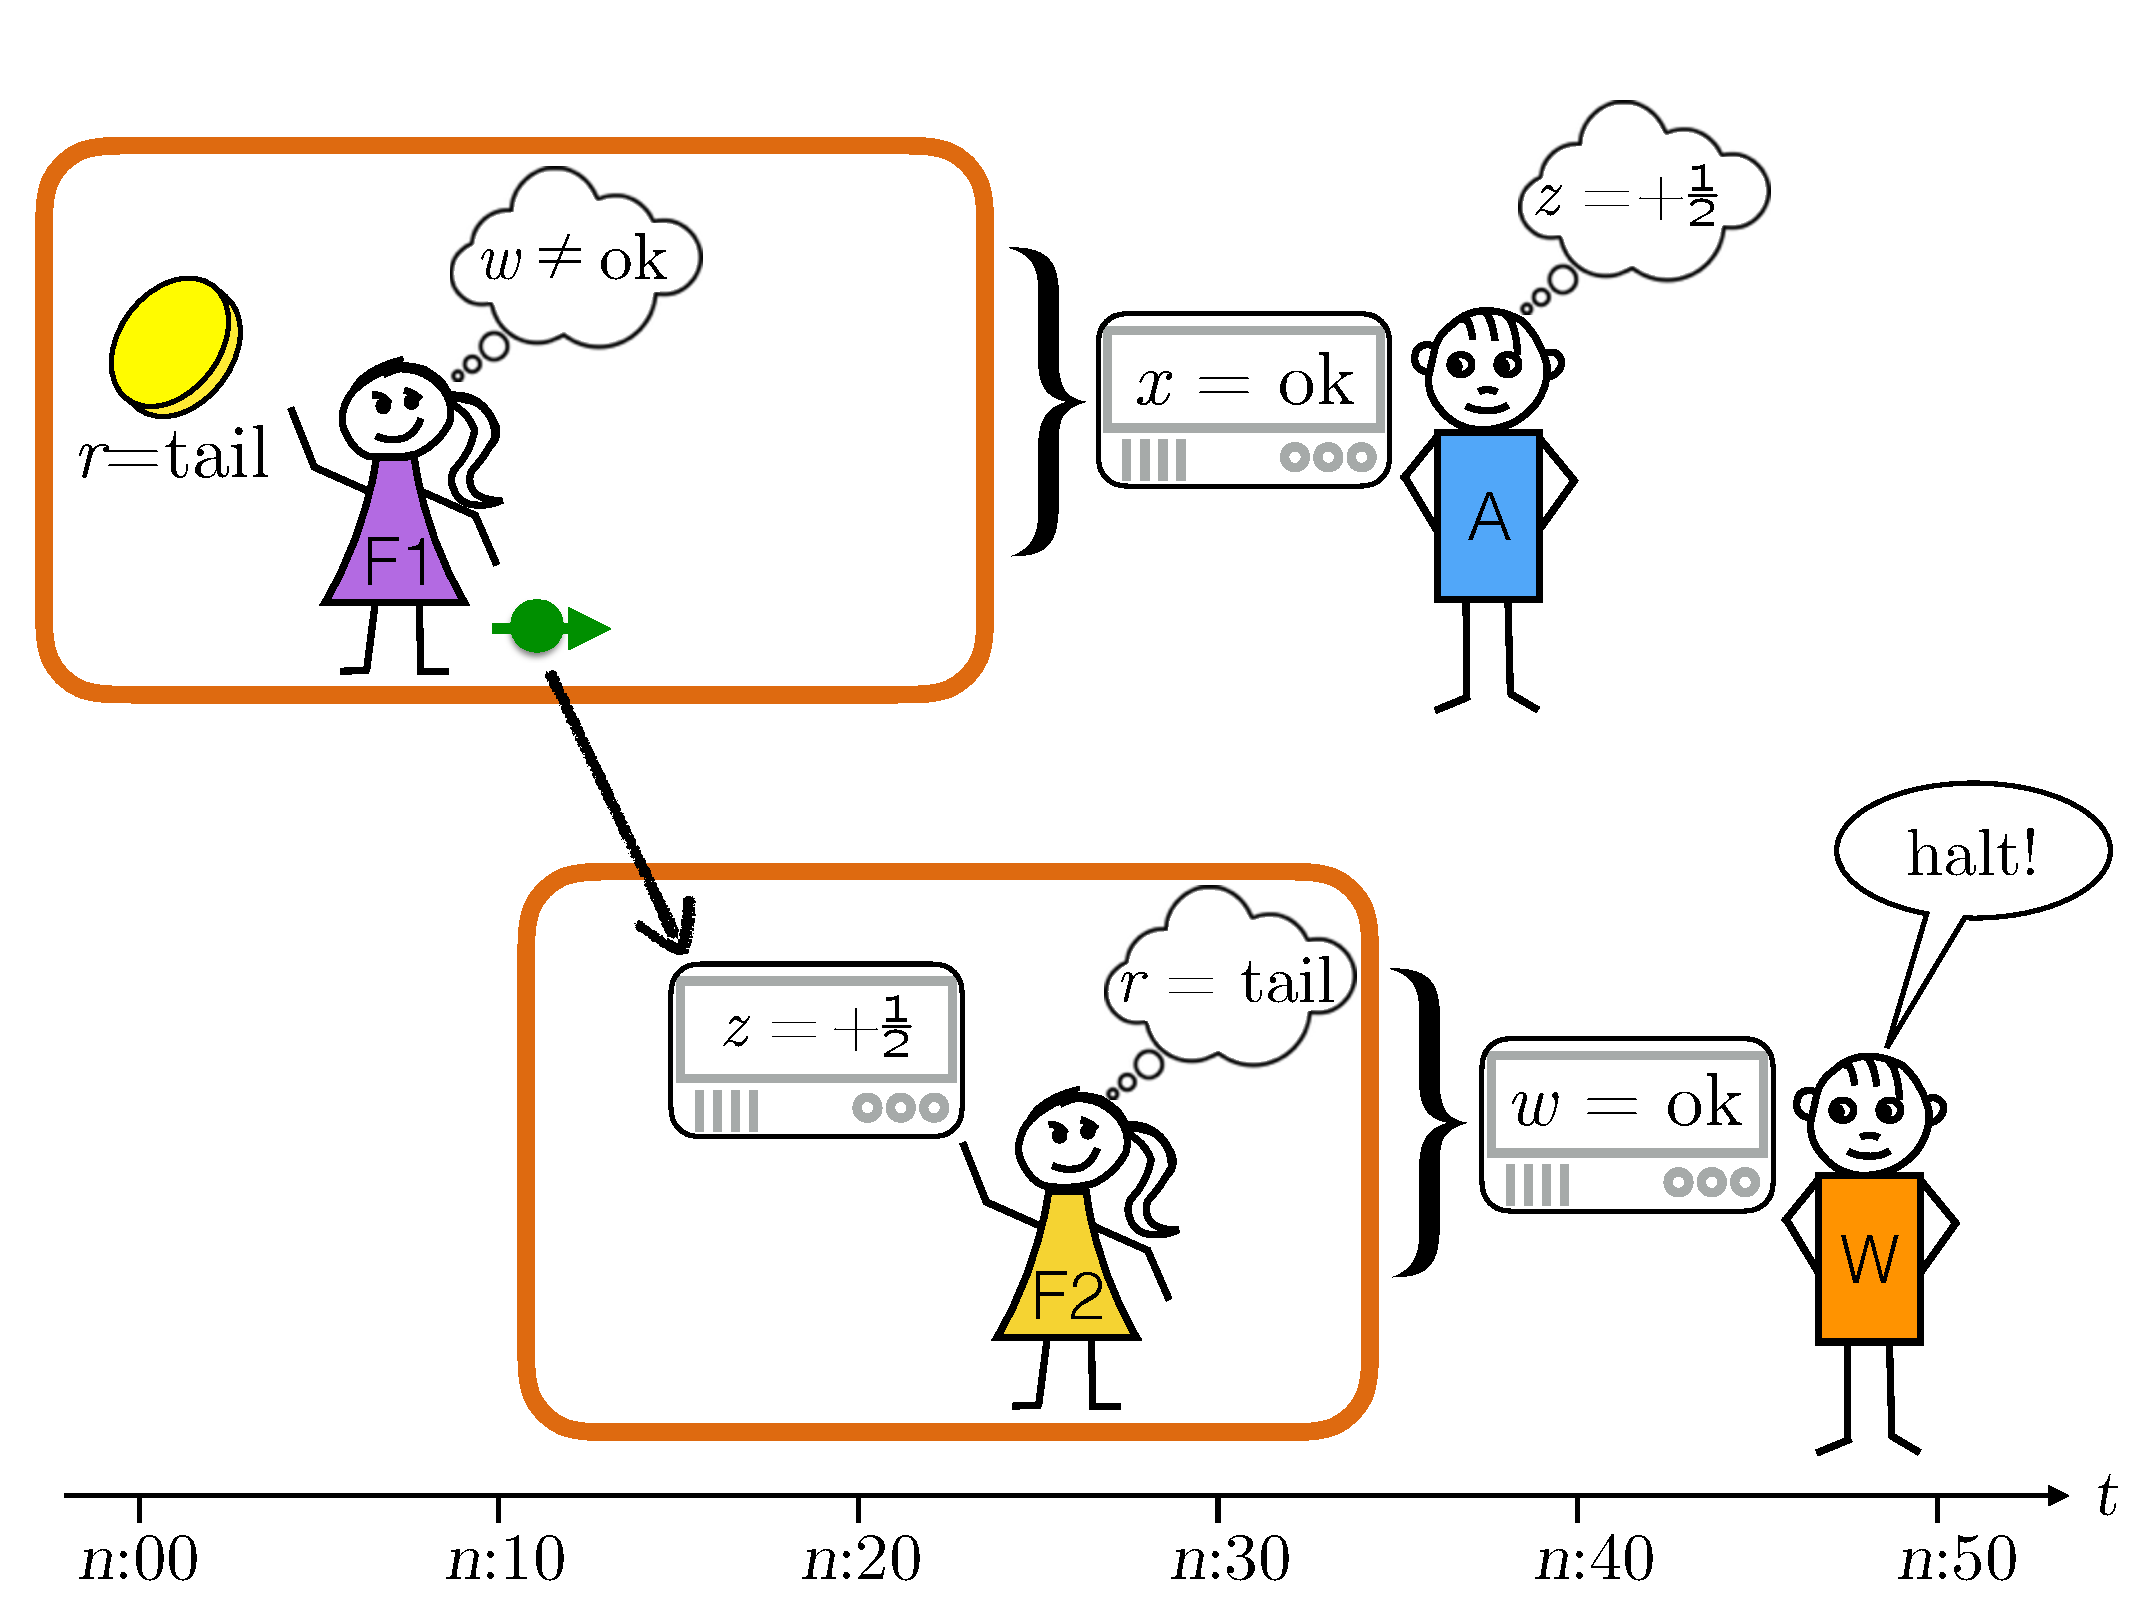
\includegraphics[trim= 0.4cm  0.2cm 0cm 1cm, clip=true, width=0.8\textwidth]{WFDiagram.pdf}
\caption{\emph{Illustration of the Extended Wigner's Friend Experiment.} In any round~$n$ of the experiment, one of Wigner's friends, $\Friendone$, polarises an electron depending on a random value~$r$. The other friend, $\Friendtwo$, measures its vertical polarisation $z$. Wigner's assistant, $\Assistant$, and Wigner, $\Wigner$, measure the entire labs of~$\Friendone$ and~$\Friendtwo$, giving outcomes $x$ and $w$, respectively. The experimenters use quantum theory to derive statements about values seen by others. $\Friendone$, for instance, tries to infer~$w$ as measured by~$\Wigner$. The experiment ends when $x = w = \ok$. 
\label{fig_EWF}
}
\end{figure}

\subsection{The experimenters' views} \label{sec_expview}

To describe the Extended Wigner's Friend Experiment formally, we subdivide it into four ``sub-experiments'', which we label by the four experimenters,  $\Friendone$, $\Friendtwo$, $\Assistant$, and $\Wigner$. The idea is that experiment $\Friendone$ is a specification of the part relevant to experimenter $\Friendone$, and so on.\footnote{This double use of notation is unproblematic as it is always clear from the context whether we mean the experimenter or the corresponding experiment.} The  idea behind this subdivision is that each of the four experiments corresponds, up to relabelings, to a Repeated Measurement Experiment, as introduced in Section~\ref{sec_QT}, and can therefore be described using standard quantum theory. Note that such a description is not possible for the joint experiment, since $z$ and $w$, for instance, cannot  simultaneously be regarded as observables according to quantum theory.

\subsubsection*{Definition of Experiment $\Friendone$}

The experimenter~$\Friendone$ prepares the state $\psi_\Spin$ of~$\Spin$ depending on the value $r$. Furthermore, we assume that she is interested in the outcome $w$ measured at time $t = \text{$n$:40}$. The corresponding event space may therefore be defined as
\begin{align}
  [\Friendone] = \,  &  \bigl\{(t, r, \psi_\Spin, w)   \in \cT \times \{\head,\tail,\bot\} \times \cH_{\Spin} \times \{\ok, \fail, \bot\} : \,  \nonumber 
  %  \\    & \quad  \text{if } t \in [\text{$n$:00}, \text{$n$:30}) \text{ then } r \neq \bot  \nonumber 
  \\  & \quad  \text{if } t  = \text{$n$:10} \text{ then } r \! = \! \head \Leftrightarrow \psi_{\Spin}\! = \! \spindown \text{ and }  r\! =\! \tail \Leftrightarrow \psi_{\Spin} \! = \! \spinright \label{eq_Fonerpsi}
  %  \\ & \quad  \text{if } t \in [\text{$n$:40}, \text{$n$:50}) \text{ then } w \neq \bot  \nonumber 
  \bigr\} \ ,
\end{align}
for $\cT$ as defined by~\eqref{eq_timeset}. 
%The plot $s^{\Friendone}$ of the story $s$ described above, for instance,  would then include the elements
%\begin{align*}
%  \begin{array}{lcl}
%  (t, \tail, \mathbf{0}, \bot)  & : &  t \in [\text{0:00}, \text{0:10}) \\
%    (t, \tail, \spinright, \bot)  & : &  t \in [\text{0:10}, \text{0:20}) \\
%  (t, \tail, \mathbf{0}, \bot) & : & t \in [\text{0:20}, \text{0:30}) \\
%  (t, \bot, \mathbf{0}, \bot)  & : & t \in [\text{0:30}, \text{0:40})  \\
%  (t, \bot, \mathbf{0}, \ok)  & : & t \in [\text{0:40},  \text{0:50}) \ ,
% \end{array}
%\end{align*}
%where we set $\psi_{\Spin} = \mathbf{0}$ for the spin state before it has been prepared and after it has been measured.
To formalise that $w$ is the outcome of a quantum measurement, we relate this experiment to one of the set $\RME_{\cH_{\Spin}, \{\pi^H_w\}}$, where $\cH_{\Spin}$ is the Hilbert space associated to the electron spin~$\Spin$ and where $\pi^H_w$ are measurement projectors in the Heisenberg picture. Specifically, taking $U = U^{\text{$n$:20}}$ (for any $n \in \mathbb{N}_0$)  to be an isometry from $\Spin$ to $\Friendtwo$ such that
\begin{align*}
  U \spindown_{\Spin}  =  \ket{\sminus}_{\Friendtwo} \qquad \text{and} \qquad
  U\spinup_{\Spin}  = \ket{\splus}_{\Friendtwo}  \ ,
\end{align*}
we define $\pi^H_{w} = U^{\dagger}  \proj{w} U$ for $w \in \{ \ok, \fail$\}. We then require that 
\begin{align} \label{eq_FriendoneM}
 \exists \,   \Exp \in \RME_{\cH_{\Spin}, \{\pi^H_w\}} : \quad  (t, *, \psi_\Spin, w) \in s^{\Friendone} \iff (t', \psi_\Spin, w) \in s^{\Exp} \ ,
\end{align}
where the mapping $t \mapsto t'$ is such that $\text{$n$:10} \mapsto \text{$n$:00}$, $\text{$n$:40} \mapsto \text{$n$:01}$, and $\text{$n$:50} \mapsto \text{$n$:02}$.   Note that this mapping must not be injective. While the time information contained in the plot $s^{\Exp}$ is thus more coarse-grained than that of $s^{\Friendone}$, it is still sufficient to apply the laws of quantum theory, as formulated by~$\QT$.

\subsubsection*{Definition of Experiment $\Friendtwo$}

Experimenter~$\Friendtwo$ measures the vertical spin direction~$z$. We assume that she is also interested in the state $\psi_\Spin$ as well as the randomness~$r$ it depends on. We therefore define the event space as
\begin{align}
  [\Friendtwo]  = \, & \bigl\{(t, r, \psi_\Spin, z)   \in \cT \times \{\head,\tail,\bot\} \times \cH_{\Spin} \times \{\sminus, \splus, \bot\} : \, \nonumber 
 %  \\ & \quad  \text{if } t \in [\text{$n$:00}, \text{$n$:30}) \text{ then } r \neq \bot \bigr\}  \nonumber 
\\  & \quad  \text{if } t = \text{$n$:10} \text{ then } r \! = \! \head \Leftrightarrow \psi_{\Spin} \! = \! \spindown \text{ and }  r \! = \! \tail \Leftrightarrow \psi_{\Spin} \! = \! \spinright  \label{eq_Ftworpsi}
 % \\ & \quad  \text{if } t \in [\text{$n$:20}, \text{$n$:40}) \text{ then } z \neq \bot  \label{eq_Ftwozbot} 
 \bigr\} \ .
  \end{align}
  To specify how $z$ arises as the outcome of a quantum measurement, we define $\pi^H_{z} = \proj{z}$  for $z \in \{\sminus, \splus\}$ and demand that  
  \begin{align} \label{eq_FriendtwoM}
 \exists \,  \Exp \in \RME_{\cH_{\Spin}, \{\pi^H_z\}} : \quad  (t, *, \psi_\Spin, z) \in s^{\Friendtwo} \iff (t', \psi_\Spin, z) \in s^{\Exp} \ ,
\end{align}
where $t \mapsto t'$ is such that $\text{$n$:10} \mapsto \text{$n$:00}$, $\text{$n$:20} \mapsto \text{$n$:01}$ and $\text{$n$:40} \mapsto \text{$n$:02}$. 

\subsubsection*{Definition of Experiment $\Assistant$}

Experimenter $\Assistant$ is measuring $x$ and, in addition, interested in the outcome~$z$ of the measurement at~$t = \text{$n$:20}$. Since these outcomes ultimately depend on the initial state $\psi_{\Coin} \in \cH_{\Coin}$ of the quantum coin $\Coin$, we also include it in the event space, which we choose to be
\begin{align}
    [\Assistant]  = \, & \bigl\{(t, \psi_{\Coin}, z, x) \in \cT \times \cH_\Coin\times \{\sminus, \splus, \bot\} \times \{\ok, \fail, \bot\} : \, \nonumber  \\ & \quad \text{if } t = \text{$n$:00} \text{ then } \psi_{\Coin} = \psi_{\Coin}^0  \label{eq_Assistantpsi} 
%   \\ & \quad \text{if } t \in [\text{$n$:20}, \text{$n$:30}] \text{ then } z \neq \bot \label{eq_Assistantzbot}   
%    \\ & \quad \text{if } t \in [\text{$n$:30}, \text{$n$:40}] \text{ then } x \neq \bot 
%    \bigr\}  \ ,
\end{align}
for $\psi^0_{\Coin}$ as defined by~\eqref{eq_Qinitialstate}. To describe this as a quantum measurement, let $V = V^{\text{$n$:00} - \text{$n$:10}}$ be an isometry from $\Coin$ to $\Friendone \otimes \Spin$  such that
\begin{align*}
  V \ket{\head}_\Coin =  \ket{\head}_{\Friendone} \otimes \spindown_{\Spin} \qquad \text{and} \qquad
  V\ket{\tail}_\Coin = \ket{\tail}_{\Friendone} \otimes \spinright_{\Spin} 
\end{align*}
and define the projectors $\pi^H_{z, x} = V^{\dagger} \proj{x} \otimes \proj{z} V$. We then require that
  \begin{align} \label{eq_AssistantM}
  \exists \,  \Exp \in \RME_{\cH_{\Coin}, \{\pi^H_{z,x}\}} : & \\
  \text{if $t = [\text{$n$:00}, \text{$n$:20}$)} : & \quad  (t, \psi_\Coin, *, *) \in s^{\Assistant} \iff \bigl(\text{$n$:00}, \psi_{\Coin}, * \bigr) \in s^{\Exp} \nonumber \\
    \text{if $t = [\text{$n$:20}, \text{$n$:30}$)} : & \quad  (t, \psi_\Coin, z, *) \in s^{\Assistant} \iff \bigl(\text{$n$:01}, \psi_{\Coin}, (z,*) \bigr) \in s^{\Exp}  \nonumber \\
    \text{if $t = [\text{$n$:30}, \text{$n$:40}$)} : & \quad  (t, \psi_\Coin, z, x) \in s^{\Assistant} \iff \bigl(\text{$n$:01}, \psi_{\Coin}, (z, x)\bigr) \in s^{\Exp} \nonumber \\
    \text{if $t = [\text{$n$:40}, \text{$n$:50}$)} : & \quad  (t, \psi_\Coin, *, x) \in s^{\Assistant} \iff \bigl(\text{$n$:01}, \psi_{\Coin}, (*, x)\bigr) \in s^{\Exp} \nonumber \ ,
\end{align}
 where we restrict to values $z \neq \bot$ and $x \neq \bot$.

%where $t \mapsto t'$ is such that $\text{$n$:00} \mapsto \text{$n$:00}$, $\text{$n$:20} \mapsto \text{$n$:01}$, $\text{$n$:30} \mapsto \text{$n$:01}$,  $\text{$n$:40} \mapsto \text{$n$:01}$, and $\text{$n$:50} \mapsto \text{$n$:02}$, and where
%\begin{align} \label{eq_Assistantzbot}   
%  z|_t = \begin{cases}
%    z & \text{if $t \in [\text{$n$:20}, \text{$n$:40})$ for some $n \in \mathbb{N}$} \\
%    \bot & \text{otherwise}
%  \end{cases}
%\end{align}
%and
%\begin{align}
%  x|_t = \begin{cases}
%    x & \text{if $t \in [\text{$n$:30}, \text{$n$:50})$ for some $n \in \mathbb{N}$} \\
%    \bot & \text{otherwise.}
%  \end{cases}
%\end{align}

\subsubsection*{Definition of Experiment $\Wigner$}

Experimenter~$\Wigner$ measures $w$ and is also interested in $x$. Similarly to the above, the event space shall therefore be
\begin{align}
      [\Wigner] = \, & \bigl\{(t, \psi_{\Coin}, x, w)  \in \cT \times \cH_\Coin \times \{\ok, \fail, \bot\} \times  \{\ok, \fail, \bot\} : \nonumber \\ & \quad \text{if } t = \text{$n$:00} \text{ then } \psi_{\Coin} = \psi_{\Coin}^0 \label{eq_Wignerpsi} \bigr\}  \ .
      %  \\ & \quad \text{if } t \in [\text{$n$:30}, \text{$n$:50}) \text{ then } y \neq \bot \nonumber
      % \\  & \quad \text{if } t \in [\text{$n$:40}, \text{$n$:50}) \text{ then } w \neq \bot  \nonumber \ .
\end{align}
To describe this as a quantum measurement, we define the projectors
\begin{align*}
  \pi^{H}_{x, w} = V^{\dagger} \proj{x} \otimes \bigl(U^{\dagger} \proj{w} U \bigr) V \ \ ,
\end{align*}
where $U$ and $V$ are the isometries from above. We then require that 
  \begin{align} \label{eq_WignerM}
 \exists \,  \Exp \in \RME_{\cH_{\Coin}, \{\pi^H_{x, w}\}} \cap \BOE:  \\ 
 \text{if $t = [\text{$n$:00}, \text{$n$:30}$)} : & \quad  (t, \psi_\Coin, *, *) \in s^{\Wigner}  \iff \bigl(\text{$n$:00}, \psi_{\Coin}, * \bigr) \in s^{\Exp} \nonumber \\ 
    \text{if $t = [\text{$n$:30}, \text{$n$:40}$)} : & \quad  (t, \psi_\Coin, x, *) \in s^{\Wigner}  \iff \bigl(\text{$n$:01}, \psi_{\Coin}, (x,*) \bigr) \in s^{\Exp}  \nonumber \\
    \text{if $t = [\text{$n$:40}, \text{$n$:50}$)} : & \quad  (t, \psi_\Coin, x, w) \in s^{\Wigner}   \iff \bigl(\text{$n$:01}, \psi_{\Coin}, (x, w)\bigr) \in s^{\Exp} \ ,\nonumber 
 %   \text{if $t = [\text{$n$:40}, \text{$n$:50}$)} : & \quad (t, \psi_\Coin, x, w) \in s^{\Wigner} \iff \bigl(\text{$n$:01}, \psi_{\Coin}, (*, x)\bigr) \in s^{\Exp} \ ,
\end{align}
where we restrict to values $x \neq \bot$ and $w \neq \bot$. 
% \quad  (t, \psi_\Coin, x, w) \in s^{\Wigner} \iff (t', \psi_{\Coin}, (x, w)) \in s^{\Exp}
%where $t \mapsto t'$ is such that $\text{$n$:00} \mapsto \text{$n$:00}$, $\text{$n$:30} \mapsto \text{$n$:00}$, $\text{$n$:40} \mapsto \text{$n$:01}$,  and $\text{$n$:50} \mapsto \text{$n$:02}$.  
Note that $\Exp \in \BOE$ ensures that the single-world property~$\SW$ holds from the viewpoint of~$\Wigner$. The condition that the experiment is repeated until the halting criterion  is satisfied (which can be tested by $\Wigner$) then corresponds to~\eqref{eq_untilhalt}, with $\hat{z} = (\ok, \ok)$. This could also be restated as
\begin{multline} \label{eq_alwaysrepeat}
    n=0   \text{ or } (\text{$(n-1)$:40}, *, x, w) \in s^{\Wigner} \text{ for $(x, w) \neq (\ok, \ok)$}  \\ \quad \implies \quad \forall \, t \in [\text{$n$:00}, \text{$n$:40}] :\,  (t, *, *, *) \in s^{\Wigner}  \ .
 \end{multline}
 By induction, it is easy to see that this condition implies that
 \begin{align}\label{eq_repetitionimplication}
   \forall \, t \in [\text{$n$:00}, \text{$n$:40}] : \,  (t, *, *, *) \in s^{\Wigner}
 \end{align}
 for any $n$ not larger than the minimum one satisfying $(\text{$n$:40}, *, x = \ok, w = \ok) \in s^{\Wigner}$.


\subsubsection*{Compatibility conditions}

The experiments $\Friendone$, $\Friendtwo$, $\Assistant$, and $\Wigner$ obviously have certain overlapping elements | after all, they are all part of one big experiment. As explained in Section~\ref{sec_views}, the overlap between the experiments can be defined via compatibility constraints. Specifically, we demand that 
\begin{align} \label{eq_compFoneWigner}
   (t, *, *, w) \in s^{\Friendone} \quad \iff \quad (t, *, *, w) \in s^{\Wigner} \ ,
\end{align}
which models that the quantity $w$ defined in the experiment $\Wigner$ is the same as the one $\Friendone$ refers to. Similarly, the compatibility constraints which model that $r$, $z$, and $x$ denote the same quantities in each experiment can be written as 
\begin{align} \label{eq_compFoneFtwo}
   (t, r, *, *) \in s^{\Friendone} \quad & \iff \quad  \, (t, r, *, *) \in s^{\Friendtwo} \\ 
   \label{eq_compFtwoAssistant}  (t, *, *, z) \in s^{\Friendtwo} \quad & \iff \quad (t, *, z, *) \in s^{\Assistant}  \\
 \label{eq_compAssistantWigner} (t, \psi_{\Coin}, *, x) \in s^{\Assistant} \quad & \iff \quad  (t, \psi_{\Coin}, x, *) \in s^{\Wigner}      \ .
\end{align}

\section{Proof} \label{sec_proof}

We split the proof of Theorem~\ref{thm_main} in two parts. In the first, we use property~$\QT$ to analyse the sub-experiments $\Friendone$, $\Friendtwo$, $\Assistant$, and $\Wigner$ separately.  We recall that each of them models a part of the Extended Wigner's Friend Experiment that is of interest to one of the four experimenters. Accordingly,  the conclusions we obtain from this analysis, \eqref{eq_QTFriendone}, \eqref{eq_QTFriendtwo},  \eqref{eq_QTAssistant}, and \eqref{eq_QTWigner}, are those that the experimenters would arrive at if they applied standard quantum theory.  Then, in the second part of the proof, we use properties $\SW$ and $\SelfCons$ to combine these individual conclusions, which then leads to a contradiction. 

\subsection{Analysis of individual views} \label{sec_analysisindividual}

For the following, let $T$ be any theory that satisfies property~$\QT$ and let $s$ be any story that is not forbidden by~$T$.

\subsubsection*{Analysis of Experiment $\Friendone$} 

 By linearity, we have
\begin{align*}
  U \spinright_\Spin 
  = U \bigl(  \sqrt{\nicefrac{1}{2}} \spindown_\Spin + \sqrt{\nicefrac{1}{2}} \spinup_\Spin \bigr) 
  = \ket{\fail}_{\Friendtwo}  \ ,
\end{align*}
which immediately implies that $\|\pi_{\fail}^H \spinright_{\Spin}\| = 1$. Hence, item~\ref{it_QMa} of property~$\QT$, which applies due to~\eqref{eq_FriendoneM},  tells us that
\begin{align*}
  (\text{$n$:10}, *, \spinright_{\Spin}, *) \in s^{\Friendone}  \quad \implies \quad  (\text{$n$:40}, *, *, w=\fail) \ .
\end{align*}
Using furthermore the constraint~\eqref{eq_Fonerpsi}, we conclude that
\begin{align} \label{eq_QTFriendone}
  (\text{$n$:10}, r=\tail, *, *) \in s^{\Friendone}  
  \quad \implies \quad
   (\text{$n$:40}, *, *, w=\fail) \in s^{\Friendone}  \ .
\end{align}

\subsubsection*{Analysis of Experiment $\Friendtwo$}  

Here $\QT$ applies because of~\eqref{eq_FriendtwoM}. Item~\ref{it_QMb} thus asserts that
\begin{align*}
   (\text{$n$:20}, *, *, z=\splus) \in s^{\Friendtwo}  \quad \implies \quad \exists \, \psi_{\Spin} : \,  (\text{$n$:10}, *, \psi_{\Spin}, *) \in s^{\Friendtwo} \text{ and } \|\pi^H_{+\frac{1}{2}} \psi_{\Spin}\| \neq 0  \ .
\end{align*}
By the constraint~\eqref{eq_Ftworpsi}, we conclude that
\begin{align} \label{eq_QTFriendtwo}
  (\text{$n$:20}, *, *, z = \splus) \in s^{\Friendtwo} \quad \implies \quad 
(\text{$n$:10}, r = \tail, *, *) \in s^{\Friendtwo} \ .
\end{align}

\subsubsection*{Analysis of Experiment $\Assistant$}  

Using the explicit form~\eqref{eq_Qinitialstate} of~$\psi^0_{\Coin}$ we find that 
\begin{align}
  V \psi^0_\Coin 
  & = \sqrt{\nicefrac{1}{3}}\ket{\head}_{\Friendone}  \otimes  \spindown_\Spin + \sqrt{\nicefrac{2}{3}} \ket{\tail}_{\Friendone}  \otimes \spinright_\Spin\nonumber \\
    & = \sqrt{\nicefrac{1}{3}}  \ket{\head}_{\Friendone} \otimes  \spindown_\Spin  + \sqrt{\nicefrac{1}{3}}   \ket{\tail}_{\Friendone}  \otimes \spindown_\Spin  + \sqrt{\nicefrac{1}{3}} \ket{\tail}_{\Friendone} \otimes  \spinup_\Spin  \nonumber \\
  & = \sqrt{\nicefrac{2}{3}}  \ket{\fail}_{\Friendone} \otimes \spindown_\Spin + \sqrt{\nicefrac{1}{3}}  \ket{\tail}_{\Friendone}  \otimes \spinup_\Spin \ . \label{eq_jointstatetwo}
\end{align}
This vector is obviously orthogonal to $\ket{\ok}_{\Friendone} \otimes \spindown_{\Spin} $.  This means that $\psi^0_{\Coin}$ is orthogonal  to~$\pi^H_{-\frac{1}{2}, \ok}$.  Furthermore, \eqref{eq_Assistantpsi} guarantees that
\begin{align*}
  (\text{$n$:00}, \psi_{\Coin}, * , *) \in s^{\Assistant} \quad \implies \quad \psi_{\Coin} = \psi^0_{\Coin} \ .
\end{align*}
Let $\Exp$ be an experiment as defined by~\eqref{eq_AssistantM}.  It follows from item~\ref{it_QMb} of~$\QT$ that
\begin{align} \label{eq_znotok}
  \bigl(\text{$n$:01}, *, (z = \sminus, x = \ok) \bigr) \notin s^{\Exp} \ .
\end{align}
By~\eqref{eq_AssistantM} we also have
\begin{multline*}
  (\text{$n$:40}, * , *, x=\ok) \in s^{\Assistant}  \quad \implies \quad 
    (\text{$n$:01}, *, (z, x = \ok)) \in s^{\Exp}  \\ \quad \implies \quad 
  (\text{$n$:20}, * , z, *) \in s^{\Assistant} 
\end{multline*}
for some value $z \neq 0$.  Since, according to~\eqref{eq_znotok}, $z \neq \sminus$, we conclude that
\begin{align} \label{eq_QTAssistant}
  (\text{$n$:40}, * , *, x=\ok) \in s^{\Assistant}  
  \quad \implies \quad
 (\text{$n$:20}, * , z=\splus, *) \in s^{\Assistant} \ .
 \end{align}

\subsubsection*{Analysis of Experiment $\Wigner$} 

Using~\eqref{eq_jointstatetwo} we find
\begin{align} \label{eq_global}
    U V \psi^0_\Coin 
  = \sqrt{\nicefrac{2}{3}} \otimes \ket{\fail}_{\Friendone} \otimes \ket{\sminus}_{\Friendtwo} 
    + \sqrt{\nicefrac{1}{3}} \otimes \ket{\tail}_{\Friendone} \otimes \ket{\splus}_{\Friendtwo} \ .
\end{align}
The overlap between this state and the state $\ket{\ok}_{\Friendone}  \otimes  \ket{\ok}_{\Friendtwo}$ equals
\begin{align*}
  \sqrt{\nicefrac{1}{3}} \spr{\ok}{\tail}_{\Friendone} \spr{\ok}{\splus}_{\Friendtwo} = \sqrt{\nicefrac{1}{12}}  \ .
\end{align*}
In other words, the state $\psi^0_{\Coin}$ has a non-zero overlap with the projector $\pi^H_{\ok, \ok}$.  Furthermore, \eqref{eq_Wignerpsi} ensures that the system is always prepared in this state, unless no state was prepared at all. Item~\ref{it_QMc} of~$\QT$, which applies due to~\eqref{eq_WignerM}, together with the requirement~\eqref{eq_alwaysrepeat} that the experiment is repeated until the halting condition is satisfied, implies that there must exist a round $n$ where  $x = w = \ok$ occur, i.e., 
\begin{align} \label{eq_QTWigner}
   (\text{$n$:40}, *, x=\ok,  w=\ok) \in s^{\Wigner} 
\end{align}
holds whenever the plot~$s^{\Wigner}$ is defined.
% holds unless $s^{\Wigner}$ is undefined.  


\subsection{Combining the views}

Assume by contradiction that $T$ satisfies the three properties $\QT$, $\SW$, and $\SelfCons$. Property $\SelfCons$ implies that there must exist a story $s$ that is not forbidden by $T$ such that all of $s^{\Friendone}$, $s^{\Friendtwo}$, $s^{\Assistant}$, and $s^{\Wigner}$ are defined. In the following we consider such a story $s$. 

According to the analysis above, there must exist a round $n$ such that~\eqref{eq_QTWigner} holds. Taking $n$ to be the smallest such number, it follows from~\eqref{eq_repetitionimplication} that
\begin{align} \label{eq_repeatimpl}
  \forall \,  t \in [\text{$n$:00}, \text{$n$:40}] :\,  (t, *, *, *) \in s^{\Wigner}  \ .
\end{align}
%Due to the compatibility constraint~\eqref{eq_compFoneWigner} this also implies that
%\begin{align*}
%  \forall t \in [\text{$n$:00}, \text{$n$:50}] :\,  (t, *, *, *) \in s^{\Friendone}  \ .
%\end{align*}
Furthermore, by virtue of~\eqref{eq_WignerM} we can apply property~$\SW$, which implies
\begin{align} \label{eq_ywsingle}
    \bigl| \bigl\{(x, w) \in \{\ok, \fail\} \times  \{\ok, \fail\}  : \,  (\text{$n$:40}, *, x, w) \in s^{\Wigner} \bigr\} \bigr| = 1 \ .
\end{align}
%This means in particular that for any $t, t' \in [\text{$n$:40}, \text{$n$:50}]$
%\begin{align} \label{eq_xWpersistence}
%  (t, *, x, w) \in s^{\Wigner} \quad \iff \quad  (t', *, x, w) \in s^{\Wigner}  \ ,
%\end{align}
%i.e., the value $x$ and $w$ remain the same within the time interval $[\text{$n$:40}, \text{$n$:50}]$. Similarly, one can argue that for any $t, t' \in [\text{$n$:30}, \text{$n$:50}]$
%\begin{align} \label{eq_xApersistence}
%  (t, *, x, *) \in s^{\Assistant} \quad \iff \quad  (t', *, x, *) \in s^{\Assistant}  \ ,
%\end{align}
%that for any $t, t' \in [\text{$n$:20}, \text{$n$:30}]$
%\begin{align} \label{eq_zFtwopersistence}
%  (t, *, *, z) \in s^{\Friendtwo} \quad \iff \quad  (t', *, *,z) \in s^{\Friendtwo}  \ ,
%\end{align}
%and that for any $t, t' \in [\text{$n$:00}, \text{$n$:20}]$
%\begin{align} \label{eq_rFonepersistence}
%  (t, r, *, *) \in s^{\Friendone} \quad \iff \quad  (t', r, *,*) \in s^{\Friendone}  \ ,
%\end{align}
Since we have chosen $n$ such that~\eqref{eq_QTWigner} holds, it follows that  
\begin{align} \label{eq_QTWignere}
  (\text{$n$:40}, *, x,  w) \in s^{\Wigner} \quad \iff \quad x = w = \ok \ .
\end{align}
Using the compatibility condition~\eqref{eq_compAssistantWigner} we obtain
\begin{align*}
  (\text{$n$:40}, *, *,  x = \ok) \in s^{\Assistant}   \ .
\end{align*} 
 Constraint~\eqref{eq_QTAssistant}, which resulted from the quantum-mechanical analysis from $\Assistant$'s viewpoint, hence implies that  
% at time  $t = \text{$n$:20}$ the value $z$ cannot be equal to~$\sminus$. But \eqref{eq_repeatimpl}, together with the compatibility condition~\eqref{eq_compAssistantWigner}, tells us that $z$ must admit some value. By the definition of the event space, \eqref{eq_Assistantzbot}, this must be a value from $\{\sminus, \splus\}$, so that
\begin{align*}
    (\text{$n$:20}, *, z=\splus,  *) \in s^{\Assistant}   \ .
\end{align*}
We now use the compatibility condition~\eqref{eq_compFtwoAssistant}  to infer that
\begin{align*}
      (\text{$n$:20}, *, z=\splus,  *) \in s^{\Friendtwo}  \ .
\end{align*}
Applying~\eqref{eq_QTFriendtwo}, which resulted from the quantum-mechanical analysis from $\Friendtwo$'s viewpoint, we obtain 
\begin{align*} 
 (\text{$n$:10}, r = \tail, *, *) \in s^{\Friendtwo} \ .
\end{align*}
Using the compatibility criterion~\eqref{eq_compFoneFtwo}, this means that 
\begin{align} \label{eq_rtail}
 (\text{$n$:10}, r=\tail, *, *) \in s^{\Friendone}  \ .
\end{align}
The quantum-mechanical analysis from $\Friendone$'s viewpoint, \eqref{eq_QTFriendone}, then gives
\begin{align*}
 (\text{$n$:40},  *, *, w=\fail) \in s^{\Friendone}  \ .
\end{align*} 
By the compatibility condition~\eqref{eq_compFoneWigner} this means that
\begin{align*}
  (\text{$n$:40}, *, *, w=\fail ) \in s^{\Wigner} \ .
\end{align*}
But this is in contradiction to~\eqref{eq_QTWignere}, which concludes the proof of Theorem~\ref{thm_main}. 





%
%
%~\eqref{eq_rM}, we can apply property~$\SW$ which implies that the value $r$ must remain the same, in the sense that
%\begin{align} \label{eq_rsingle}
%  \bigl| \{r: \,  (t, r, *, *) \in s^{\Friendone} \text{ for } t \in [\text{$n$:00}, \text{$n$:29}]\} \bigr| = 1 \ .
%\end{align}
%%Using the compatibility constraint~\eqref{eq_compFoneFtwo}, we also obtain
%%\begin{align*}
%%  \bigl| \{r: \,  (t, r, *, *) \in s^{\Friendtwo} \text{ for } t \in [\text{$n$:00}, \text{$n$:30}]\} \bigr| = 1 \ .
%%\end{align*}
%A similar argument shows that
%\begin{align} \label{eq_zsingle}
%  \bigl| \{z: \,  (t, *, *, z) \in s^{\Friendtwo} \text{ for } t \in [\text{$n$:20}, \text{$n$:39}]\} \bigr| = 1
%\end{align}
%and\begin{align} \label{eq_zysingle}
%    \bigl| \{(z, x): \,  (t, *, z, x) \in s^{\Assistant} \text{ for } t \in [\text{$n$:30}, \text{$n$:50}]\} \bigr| = 1 
%\end{align}
%and
%%\begin{align} \label{eq_ywsingle}
%%    \bigl| \{(x, w): \,  (t, *, x, w) \in s^{\Wigner} \text{ for } t \in [\text{$n$:40}, \text{$n$:50}]\} \bigr| = 1 \ .
%%\end{align}
%
%Since we have chosen $n$ such that~\eqref{eq_QTWigner} holds, condition~\eqref{eq_ywsingle} implies 
%\begin{align} \label{eq_QTWignere}
%  (\text{$n$:50}, *, x=\ok,  w=\ok) \in s^{\Wigner}  \ .
%\end{align}
%The compatibility condition~\eqref{eq_compAssistantWigner}, which asserts that $\Wigner$ and $\Assistant$ see the same value $x$, implies 
%\begin{align*}
%  (\text{$n$:50}, *, *,  x=\ok) \in s^{\Assistant} \ .
%\end{align*} 
%From~\eqref{eq_zysingle}, we conclude that
%%\begin{align*}
%%    (\text{$n$:30}, *, *,  x=\fail) \notin s^{\Assistant} \ .
%%\end{align*}
%%Also, because of~\eqref{eq_BMEeventsgen}, which is applied via~\eqref{eq_AssistantM} and~\eqref{eq_ObsMeas}, the measurement outcome $x$ cannot admit the value $\bot$  at time $t = \text{$n$:30}$. Using once again~\eqref{eq_zysingle}, we thus obtain
%\begin{align*}
%  (\text{$n$:30}, *, *,  x=\ok) \in s^{\Assistant} \ .
%\end{align*} 
%Similarly, the measurement outcome $z$ cannot admit the value~$\bot$ at time $t = \text{$n$:30}$. Constraint~\eqref{eq_QTAssistant}, which resulted from the quantum-mechanical analysis from $\Assistant$'s viewpoint, hence implies that the $z$ value must be equal to~$\splus$, i.e., 
%\begin{align*}
%  (\text{$n$:30}, *, z= \splus, x=\ok) \in s^{\Assistant} \ .
%\end{align*}
%The compatibility condition~\eqref{eq_compFtwoAssistant}, according to which $\Assistant$ and $\Friendtwo$ see the same value $z$, implies that
%\begin{align*}
%  (\text{$n$:30}, *, *, z=\splus) \in s^{\Friendtwo} \ .
%\end{align*}
%We now use~\eqref{eq_zsingle} to infer that
%\begin{align*}
%    (\text{$n$:20}, *, *, z=\splus) \in s^{\Friendtwo} \ .
%\end{align*}
%Applying~\eqref{eq_QTFriendtwo}, which resulted from the quantum-mechanical analysis from $\Friendtwo$'s viewpoint, we obtain
%\begin{align*}
% (\text{$n$:10}, r=\tail, *, *) \in s^{\Friendtwo} \ .
%\end{align*}
%The compatibility condition~\eqref{eq_compFoneFtwo}, which asserts that $\Friendtwo$ and $\Friendone$ see the same value $r$, implies
%\begin{align*}
% (\text{$n$:10}, r=\tail, *, *) \in s^{\Friendone}  \ .
%\end{align*}
%Using~\eqref{eq_rsingle} we find that this is equivalent to
%\begin{align} \label{eq_rhead}
% (\text{$n$:10}, r=\head, *, *) \notin s^{\Friendone}  \ .
%\end{align}
%Conversely, starting again from~\eqref{eq_QTWignere}, we can employ~\eqref{eq_ywsingle} to obtain
%\begin{align*}
%  (\text{$n$:40}, *, x=\ok,  w=\ok) \in s^{\Wigner}  \ .
%\end{align*}
%Then we can use the compatibility condition~\eqref{eq_compFoneWigner}, which ensures that  $\Friendone$ and $\Wigner$ talk about the same value $w$, to obtain
%\begin{align*}
%  (\text{$n$:40}, *, *, w = \ok) \in s^{\Friendone} \ .
%\end{align*}
%However, this and~\eqref{eq_rhead}, taken together, are in contradiction to~\eqref{eq_QTFriendone}, which was the result of the quantum-mechanical analysis from $\Friendone$'s viewpoint. This concludes the proof of Theorem~\ref{thm_main}. 

%\section{Experimental testability} \label{sec_Exp}
%
%Property~$\QT$ is used in the proof of Theorem~\ref{thm_main} to derive the relations~\eqref{eq_QTFriendone}, \eqref{eq_QTFriendtwo}, \eqref{eq_QTAssistant}, and \eqref{eq_QTWigner}.  At first glance, it seems that these relations could be experimentally tested, at least in principle, by running the Extended Wigner's Friend Experiment. Relation~\eqref{eq_QTAssistant}, for instance, could be checked by stopping the experiment shortly after time $t = \text{$n$:30}$ and comparing the values $z$ and $x$. A similar test is also possible for the other relations, except for~\eqref{eq_QTFriendone}. The problem with the latter is that it involves both $w$ and $r$. However, at time $t = \text{$n$:40}$, when $w$ is measured, $r$ may no longer be available, for this value is held by $\Friendone$, who is herself subject to a measurement at time $t = \text{$n$:30}$. 
%
%%To enable experimental verification, we need to make the additional assumption that the statements that we obtain by using a theory~$T$ are \emph{reliable}, in the sense that they should not depend on whether we actually verify them. Under this assumption, 
%
%Experimental tests are however still possible if one makes an additional, arguably rather natural, assumption, which we term \emph{reliability}.  Roughly, it demands that the statements that we obtain by using a theory~$T$ do not depend on our ability to verify them. This can be phrased more precisely in terms of stories about a general measurement experiment $\Exp \in \RME_{\cH, \{\pi^H_z\}}$ of the type introduced in Section~\ref{sec_QT}. Here reliability should mean that the measurement outcomes $z$ do not depend on whether or not the experimenter memorises what state $\psi$ the system was prepared in. More precisely, suppose that $s$ is a story according to which the initially prepared state $\psi$ is not stored. Let furthermore $\bar{s}$ be another story according to which the same outcomes occur, i.e., 
%  \begin{align} \label{eq_sameoutcomes}
%     (t, *, z)  \in s^{\Exp} \quad & \iff \quad  (t, *, z) \in \bar{s}^{\Exp}  \ ,
%  \end{align}
%but where a description of the state $\psi$ remains recorded until the measurement is carried out, i.e., 
%\begin{align} \label{eq_recordpsi}
%     (\text{$n$:00}, \psi, *)  \in s^{\Exp} \quad & \iff \quad  \forall t \in [\text{$n$:00}, \text{$n$:02}] : \, (t, \psi, *) \in \bar{s}^{\Exp}  \ .
%\end{align}
%Reliability then demands that $s$ can always be replaced by $\bar{s}$. This motivates the following definition. 
%
%%Formally, the requirement is that for any $\Exp \in \mathcal{\bar{Q}}$ the equivalence
%%\begin{align*}
%%  (\text{$n$:00}, \psi, *) \in s^{\Exp} \quad \iff \quad \forall t \in [\text{$n$:00}, \text{$n$:02}] : \, (t, \psi, *) \in s^{\Exp} 
%%\end{align*}
%%holds. 
%
%\begin{shaded}
%  \noindent When we say that a physical theory \emph{$T$ satisfies $\Reliability$} then this means that for any experiment $\Exp \in \RME_{\cH, \{\pi_z\}_z}$ and any non-forbidden story $s$ there exists a non-forbidden story $\bar{s}$ that reports the same measurement outcomes whereas a description of the prepared state $\psi$ is kept until the corresponding measurements are completed, i.e., \eqref{eq_sameoutcomes} and~\eqref{eq_recordpsi} hold.
%\end{shaded} 
%
%Suppose that one runs a modification of the Extended Wigner's Friend Experiment where  the measurement by $\Assistant$ at time $t = \text{$n$:30}$ is sometimes omitted. Instead, at time $t = \text{$n$:40}$,  the state $\psi$ held by $\Friendone$ is compared to the value $w$ measured by $\Wigner$. If the event that $\psi = \spinright$ (corresponding to $r = \tail$) and $w = \ok$ never occurs one may conclude that stories $\bar{s}$ such that 
%\begin{align} \label{eq_exptestrw}
%     (\text{$n$:40}, *, r =\tail, w=\ok) \in \bar{s}^{\Friendone} 
%\end{align}
%for any $n$ are forbidden. Property~$\Reliability$ would then imply that also any story $s$ about the unmodified Extended Wigner's Friend Experiment where
%\begin{align*}
%  (\text{$n$:10}, r=\tail, *, *) \in s^{\Friendone} \quad \text{and} \quad
%   (\text{$n$:40}, *, *, w=\ok) \in s^{\Friendone} \ .
% \end{align*}
%are also forbidden, which would imply relation~\eqref{eq_QTFriendone}. 
%
%As already noted above, the other relevant relations, \eqref{eq_QTFriendtwo}, \eqref{eq_QTAssistant}, and \eqref{eq_QTWigner}, can be tested directly. Suppose now that an experiment that tests these as well as~\eqref{eq_exptestrw} confirms these relations.  This would lead to the conclusion that no physical theory $T$ compatible with these experimental findings can have all of the properties $\SW$, $\SelfCons$, and $\Reliability$.  In other words, we would either need to give up any single-world interpretation or, alternatively, deny the possibility of describing nature with a self-consistent and reliable theory. 
%


\section{Possible scenarios} \label{sec_discussion}

According to Theorem~\ref{thm_main}, if one wishes to devise a physical theory, one has to give up at least one of the assumptions~$\QT$, $\SW$, or $\SelfCons$.  In the following three subsections, we discuss possible scenarios that arise when one of the assumptions is abandoned. They usually correspond to theories that have been proposed in the literature. The fourth subsection addresses the question whether there are other implicit assumptions built into the framework used here. 


\subsection{Theories that violate~$\QT$} \label{sec_vQT}

Property~$\QT$ demands that the laws of quantum theory are valid even for systems that are complex enough to contain an observer (who herself applies quantum theory to describe a system in her possession). This assumption is generally violated by theories that postulate a modification of the usual Schr\"odinger equation~\cite{GisRig95,Weinberg12}. Examples include spontaneous collapse models such as the GRW theory and extensions thereof~\cite{GhRiWe86,Pearle89,Tumulka06}, as well as gravity induced collapse models~\cite{Karolyhazy66,Diosi89,Penrose96} (see~\cite{Bassietal13} for a review). The same is true for the proposal of~\cite{AufGra15} to supplement the basic formalism of quantum theory with the postulate that measurements must be carried out in a context (which may include the measurement device). Since, according to the postulate, this context cannot be treated itself as a quantum system, it rules out the possibility of applying quantum measurements to measurement devices, thus violating~$\QT$. 



%``Nothing like that occurs in the CSM ontology, because it is postulated from the beginning that a measurement carried out in a given context on a system with N exclusive modalities can only give one of these modalities,''

Conversely, property~$\QT$ is not usually violated by hidden variable theories. The reason is that~$\QT$ only refers to statements that can be made with certainty within quantum theory. In particular, it does not impose any constraints on the statistics of measurement outcomes, and hence it does not rule out theories that provide more informative predictions than quantum theory~\cite{ColRen11}.  To illustrate this, one may take a variant of Bohmian mechanics where the particle positions are known. This theory, although being deterministic, would never predict an outcome that is forbidden by quantum theory, and hence still satisfy~$\QT$.

\subsection{Theories that violate~$\SW$} \label{sec_vSW}

Property~$\SW$ demands that only one single outcome occurs when we measure a quantum system. It captures the intuition that the outcome we are aware of is the only real one. Probably the most prominent representative of a theory which abandons this intuition is the relative state formalism, which is also known as the many-worlds or the Everett interpretation~\cite{Everett57,Wheeler57,DeWitt70,Deutsch85,Deutsch97,Vaidman16}. It proclaims that  the measurement of a quantum system results in a branching into different ``worlds'', in each of which one of the possible measurement outcomes occurs. The different outcomes are therefore all equally ``real'', corresponding to statement~\eqref{MWClaim} in the case of our introductory example of a spin measurement (cf.\ Fig.~\ref{fig_MW}). 

Various variants and extensions of the relative state formalism have been proposed. Among them are the many-minds interpretation~\cite{Zeh70, AlbLoe88} and the parallel lives theory~\cite{Brassard13}, as well as notions such as quantum Darwinism~\cite{Zurek07}. Their common feature is that they do not postulate a physical mechanism that singles out one particular measurement outcome, although observers have the perception of single outcomes. They are therefore all examples of theories that are not single-world in the sense of~$\SW$. 

\begin{figure}[t]
\centering
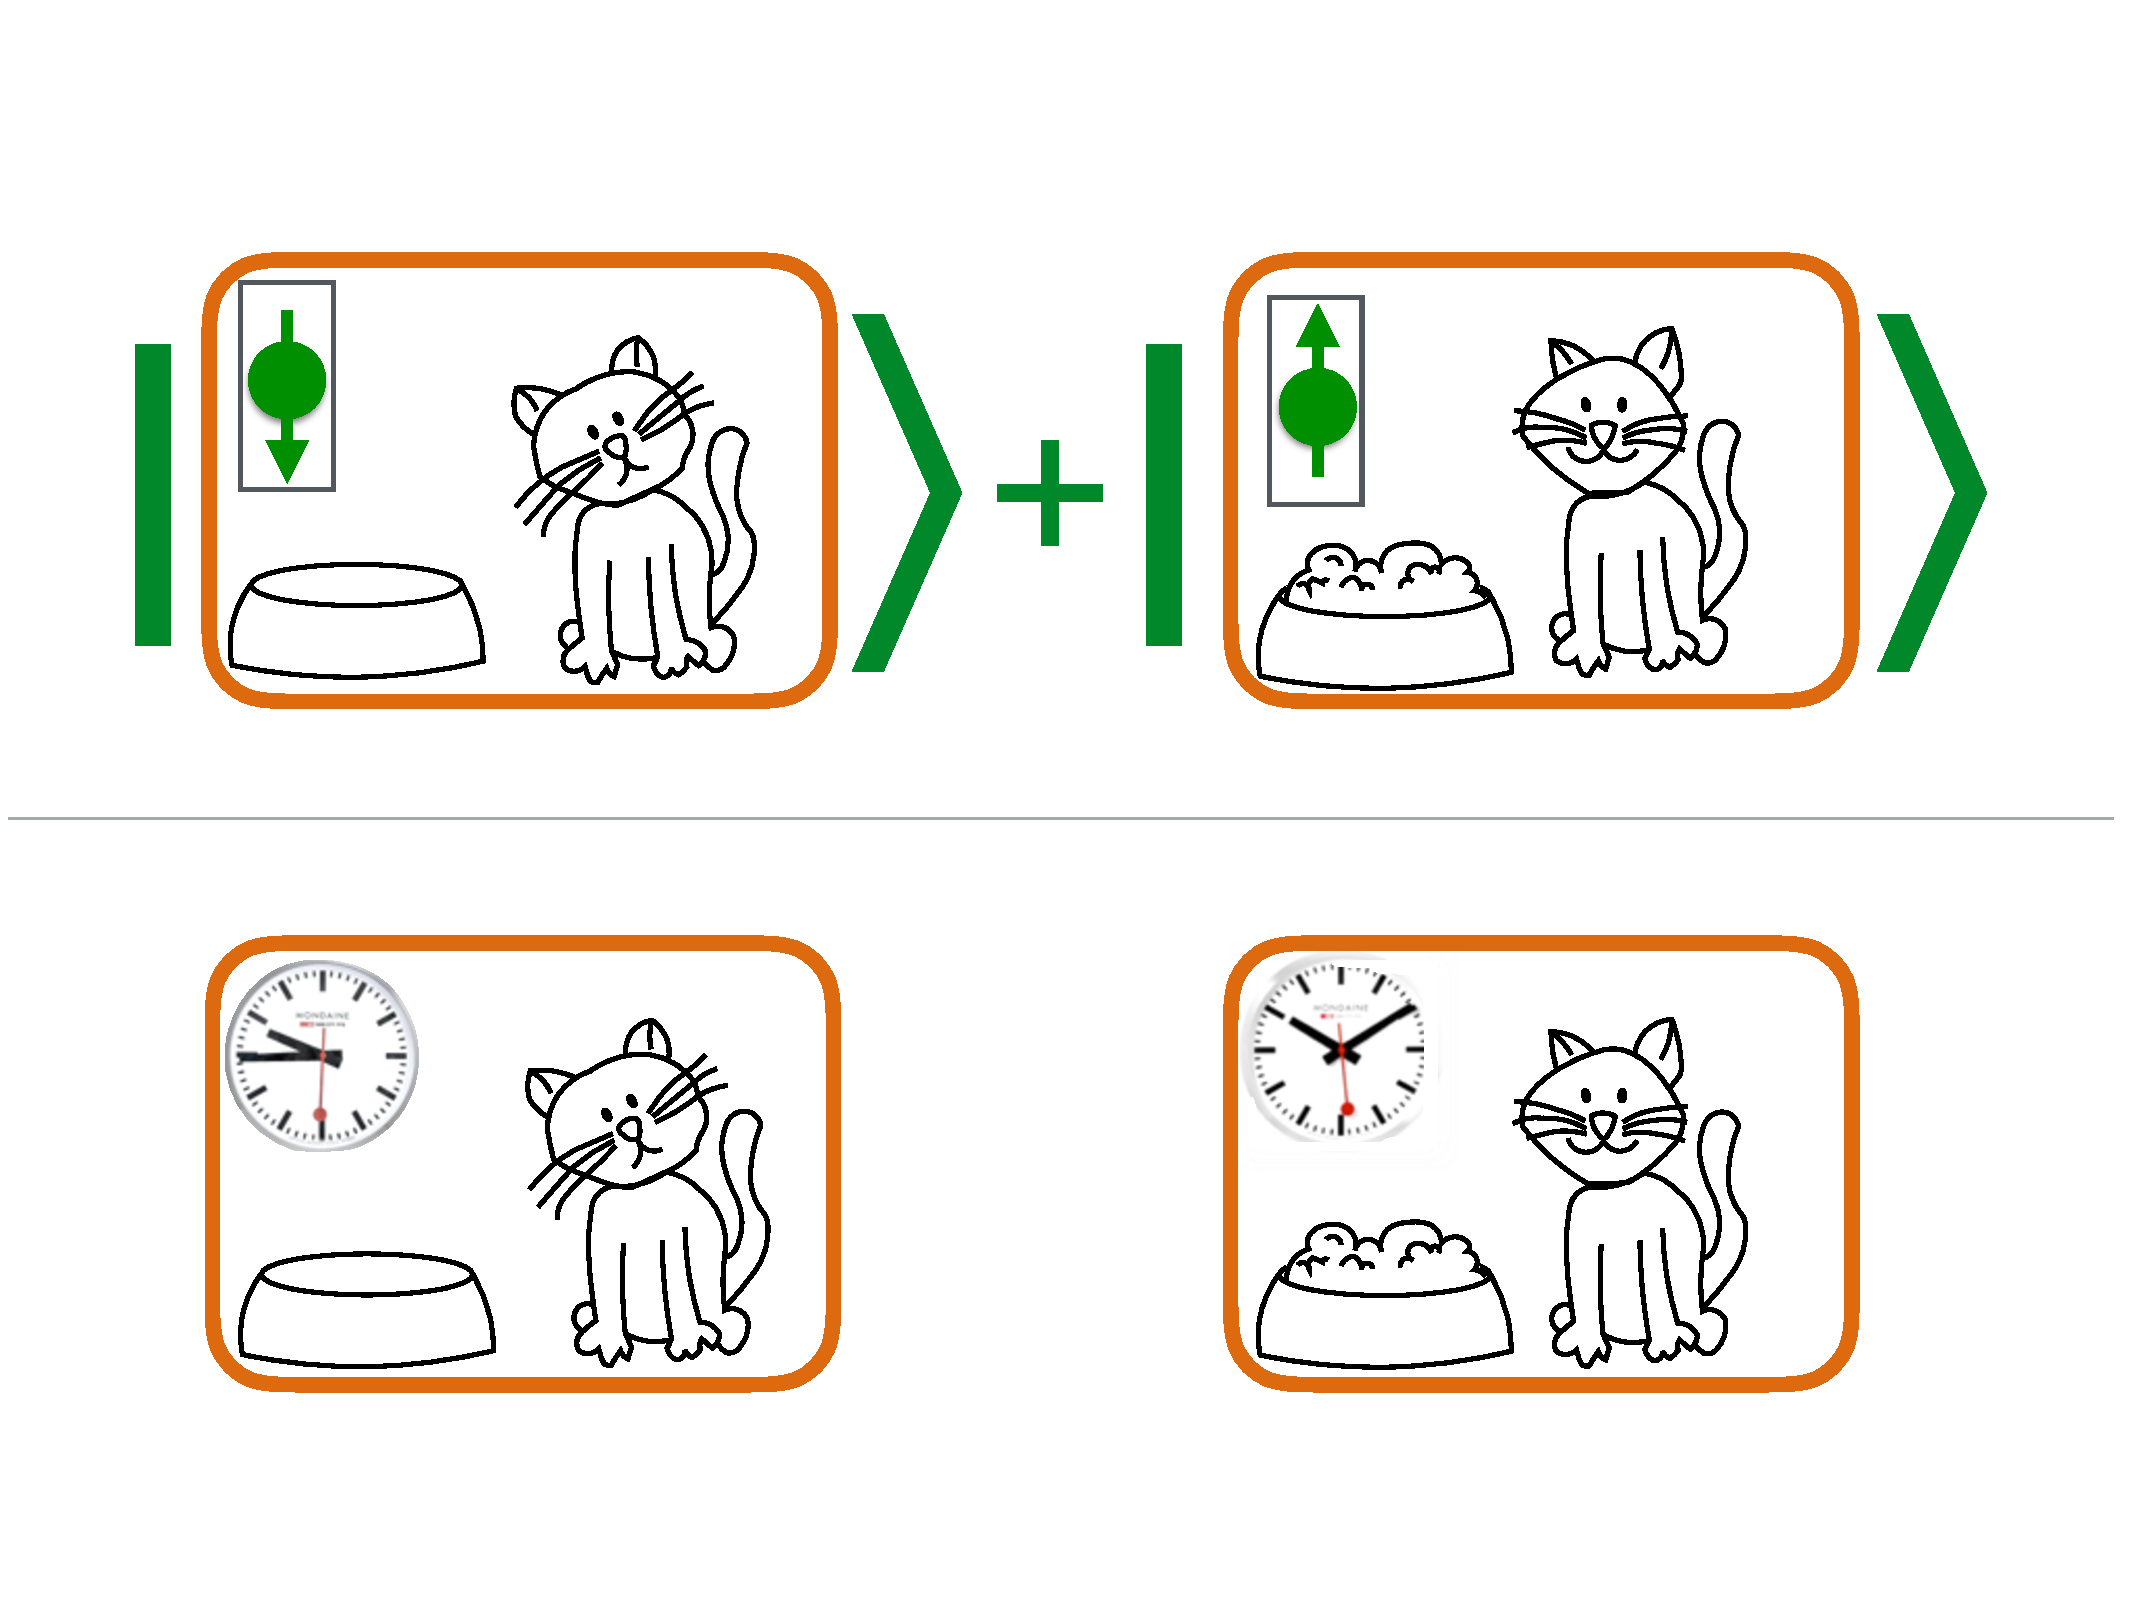
\includegraphics[trim= 0.4cm  0.2cm 1cm 4cm, clip=true, width=0.8\textwidth]{ManyWorldsTime.pdf}
\caption{\emph{The intuition behind many-worlds.}   Slightly varying the Schr\"odinger's cat gedankenexperiment~\cite{Schroedinger35},  a mechanism may decide, based on the outcome of a spin measurement, whether or not the cat is fed. According to a many-worlds interpretation, the two perceptions of the cat, hungry and happy, are equally real. While this may sound counter-intuitive, a much more familiar situation is obtained when the feeding mechanism is replaced by one triggered by time.  Assuming the cat has no good memory, the situation remains the same for her: the two perceptions, hungry and happy, are equally real.
\label{fig_MW}
}
\end{figure}

We recall, however, that property~$\SW$ does not demand that one can simultaneously assign unique outcomes to \emph{any} measurement made during an experiment. Rather, the requirement is  that  the measurement outcomes accessible to \emph{one} observer (in our case experimenter $\Wigner$) have single values.  Our analysis of the Extended Wigner's Friend Experiment therefore leads to a conclusion that differs, for instance, from that of~\cite{Brukner15}, who argued that facts cannot exist ``per se'', but that they may still exist ``relative to observers''.  Theorem~\ref{thm_main} also excludes this latter possibility. 


\subsection{Theories that violate~$\SelfCons$}

It is a consequence of Theorem~\ref{thm_main} that deterministic hidden variable theories must violate property~$\SelfCons$, i.e., they cannot be self-consistent. Indeed, as argued in Section~\ref{sec_vQT}, they satisfy~$\QT$, and because they are (by definition) deterministic, measurements have only one single outcome, so that~$\SW$ holds. 

An example of such a hidden variable theory is Bohmian mechanics. The conclusion that Bohmian mechanics is not self-consistent may be compared to the results of~\cite{CorMor02,KiuWer10}. They suggest that, in an experiment with entangled particles, the behaviour of the Bohmian particle positions  is not consistent with the statistics that quantum theory would predict for position measurements.  However, since Bohmian particle positions cannot in general be identified with the outcomes of position measurements~\cite{ESSW92,Vaidman05}, this finding does not point to a fundamental inconsistency of Bohmian mechanics~\cite{Gisin15}. This is in  contrast to the conclusions we can draw from Theorem~\ref{thm_main}, which shows that an inconsistency arises independently of how one interprets the Bohmian particle positions.

%It is instructive to explore in a bit more detail what a violation of self-consistency means in the specific case of Bohmian mechanics. For this, we may consider the Extended Wigner's Friend Experiment. One may then on the one hand  apply the theory from a more global perspective, in the same way as this is done in Section~\ref{sec_analysisindividual} for the analysis of $\Wigner$'s viewpoint, to infer that there must be a round in which $x = w = \ok$. Extending this analysis to include $z$ and $r$, one would also find that $x = \ok \implies z = \splus$ and $z = \splus \implies r = \tail$, corresponding to~\eqref{eq_QTAssistant} and~\eqref{eq_QTFriendtwo}, respectively. On the other hand, one may apply the theory from the perspective of $\Friendone$, which would lead to the conclusion that $w = \ok \implies r = \head$, corresponding to~\eqref{eq_QTFriendone}. Analysing the experiment from the two perspectives thus leads to contradicting statements about the value of~$r$.  

It is certainly unsatisfactory if a theory is not self-consistent. One may therefore ask whether there is an easy fix. One  possibility could be to restrict the range of applicability of the theory and add the rule that its predictions are only valid if an experimenter who makes the predictions keeps all relevant information stored.  While we do not normally impose such a rule when using theories to make predictions, this would, at least in the case of Bohmian mechanics, remove the inconsistency. Indeed, since in the Extended Wigner's Friend Experiment $\Friendone$ may not be able to store the value~$r$ until $t=\text{$n$:40}$, the theory could no longer be applied to analyse her part of the experiment. Formally, this means that~\eqref{eq_FriendoneM} would no longer be a valid requirement and, hence, \eqref{eq_QTFriendone} could not be established. 



\subsection{Relaxing the notion of a physical theory} \label{sec_theories}

The formulation of Theorem~\ref{thm_main} is based on a  framework, as outlined in Section~\ref{sec_framework}, which allows us to reason about \emph{physical theories}. Hence, any structure imposed by the framework potentially limits the generality of the claim. One may therefore try to further relax it. However, compared to other frameworks used in the literature on the foundations of quantum theory, the one used here is already rather minimalistic. In particular, it is not demand that a physical theory provides predictions that can be expressed in terms of probability distributions. 

To illustrate this, it is instructive to have a quick look at other approaches, such as the one taken by Bell~\cite{Bell66}. The assumptions that enter Bell's theorem are usually formulated in terms of probability distributions of certain random variables that model the outcomes of measurements.  The model therefore comes with the a priori assumption that all measurements, even if they are carried out by different experimenters, have a well-defined outcome (the value of the random variable), and that a physical theory allows us to calculate predictions (the probability distributions assigned to these variables). The same holds true for various results based on probabilistic frameworks~\cite{Barrett07,BarWil16} (cf.\ \cite{Hardy11,ChDaPe11,MasMul11,ColRen12,PuBaRu12,OrCoBr12,LeiSpe13} for some recent examples). In contrast to this, Theorem~\ref{thm_main} completely avoids the use of the notion of probability, so that no such assumption is necessary. 

One may now ask whether there are still other assumptions built into the framework used here. For example, the idea of considering multiple experimenters, which is central to our argument,  could be problematic if one takes a more radical subjective viewpoint. A nice example is QBism, according to which probabilities represent beliefs of an agent and are therefore entirely subjective~\cite{FuMeSc14}. Even if an agent assigns probability~$1$ to a particular outcome of a measurement, this should  not be taken as a fact, and QBism would even allow that another agent assigns probability~$0$ to the same outcome. This suggests that, within QBism, it may not be sensible to carry out an analysis that is based on the combination of different experimenters' views. Nevertheless, since it is rather common that we try to infer the behaviour of others by reasoning about their decision-making, it could still be interesting to explore  how QBism should be applied to situations where one agent uses QBism to express his believes about another agent's actions who herself applies QBism.  We leave a study of the  Extended Wigner's Friend Experiment from such a  Bayesian viewpoint to future research. 

\section{Conclusions} \label{sec_conclusions}

A natural requirement to any reasonable physical theory~$T$ is that different observers who apply~$T$ should not arrive at logically contradicting statements.  This is captured by property~$\SelfCons$, which demands that there exists at least one possible story~$s$ that none of the different observers would consider as forbidden.  Once one accepts~$\SelfCons$  as an unavoidable requirement, our main result, Theorem~\ref{thm_main} implies that we are left with the option to either deny~$\QT$ or~$\SW$. 

It is in principle possible to decide between these two options by an appropriately designed experiment. The experiment that would need to be carried out is a test whether the predictions of standard quantum theory are valid for systems that are complex enough to count as observers. As famously noted by Bell, defining precisely what this means appears to be impossible~\cite{Bell90}. However, experiments that test quantum coherence for macroscopic systems~\cite{ArnHor14} certainly provide evidence in favour of~$\QT$, and hence against $\SW$.

While the ultimate experiment would involve human observers, one could argue that it is sufficient to consider systems that have the same   level of complexity.  This could be achieved  once we are able to build scalable quantum computers.\footnote{Scalability means that arbitrarily complex computing devices can be built from elementary components by composition.}  Theorem~\ref{thm_main} therefore provides another incentive to build such machines. If they  work according to the predictions of quantum theory, we know we are left with Scenario~2 described in the introduction. That is, we are forced to give up the view that there is one single reality. 


\section*{Acknowledgments}

We would like to thank Alexia Auff\`eves, Serguei Beloussov, Hans Briegel, L\'idia del Rio, David Deutsch, Artur Ekert,  Nicolas Gisin, Philippe Grangier, Thomas M\"uller, Sandu Popescu, R\"udiger Schack, and Vlatko Vedral for discussing ideas that led to this work. This project was supported by the Stellenbosch Institute for Advanced Study (STIAS), by the Swiss National Science Foundation (SNSF) via the National Centre of Competence in Research ``QSIT'', by the European Research Council (ERC) via grant No.\ 258932,  and by the European Commission via the project ``RAQUEL''.  

%\appendix
%
%\section*{Appendix}
%
%\subsection*{A note on the traceless erasure of information}
%
%The measurement applied by $\Assistant$ and $\Wigner$ can be regarded as erasure maps. 
%
%We describe here a way to physically ``erase'' information such that no traces remain. To explain what we mean by this, we consider an experiment that our quantum physicist, Wigner, could carry out with his two friends, Alice and Bob. Let $X$ be a register held by Alice, which stores a value from a set $\cX$.  Assuming that Wigner knows everything about the experiment, the global state he would associate to $X$ and the relevant environment $E$ (which may include all other information held by Alice and Bob) can most generally be written as
%\begin{align*}
%  \ket{\psi}_{X E} = \sum_{x \in \cX} \sqrt{p_x} \ket{x}_X \otimes \ket{\psi^x}_E \ ,
%\end{align*}
%where $\{p_x\}_{x \in \cX}$ is a probability distribution, $\{\ket{x}_X\}_{x \in \cX}$ is an orthonormal basis, and $\ket{\psi_x}_E$ arbitrary normalised vectors on $E$.  Suppose now that, during the course of the experiment, Alice provides a copy $\bar{X}$ of $X$ to Bob. From Wigner's viewpoint, the state then has the form
%\begin{align*}
%    \ket{\psi'}_{X \bar{X} E} = \sum_{x \in \cX} \sqrt{p_x} \ket{x}_X \otimes \ket{x}_{\bar{X}} \otimes \ket{\psi^x}_E \ .
%\end{align*}
%We would now say that Bob can ``tracelessly erase'' his copy $\bar{X}$ if he | without involving Alice | can do something with the effect that the global state of $X$ and $E$, as seen from Wigner's perspective, is returned to the initial state $\ket{\psi}_{X E}$.
%
%We first note that the reduction of the state $\ket{\psi'}_{X \bar{X} E}$ on $X$ and $E$  is generally mixed. This immediately implies that it is impossible for Bob to deterministically erase $\bar{X}$ tracelessly, in the sense described above.\footnote{This fact is sometimes called the ``quantum no-deleting theorem''.}  However, there is still a way to achieve this non-deterministically. The idea is that Bob applies a projective measurement, of which one projector is along the vector
%\begin{align} \label{eq_projstate}
%  \sqrt{\nicefrac{1}{|\cX|}} \sum_{x \in \cX} \ket{x}_{\bar{X}} \ .
%\end{align}
%It is  straightforward to verify that the outcome corresponding to this projector occurs with probability $\nicefrac{1}{|\cX|}$. Furthermore, once Wigner is informed about this event, the global state from his perspective is again equal to the state $\ket{\psi}_{X E}$ we had initially. 
%
%This idea may be formulated as a little lemma.
%
%\begin{lemma}[Traceless Information Erasure]
%  Let $\cC_{X \bar{X} \leftarrow X}$ be a TPCPM that (coherently) copies information encoded w.r.t.\ an orthonormal basis $\ket{x}_{x \in \cX}$ from a system $X$ to a system $\bar{X}$, i.e., 
%  \begin{align*}
%    \cC_{X \bar{X} \leftarrow X}  : \quad \sigma_X \mapsto \sum_{x, x' \in \cX}  \bra{x} \sigma_X \ket{x'}  \bigl(\ket{x} \bra{x'}\bigr)_{X}  \otimes \bigl(\ket{x}\bra{x'} \bigr)_{\bar{X}} \ .
%  \end{align*}
%  Let furthermore $\cE_{\mathbb{C} \leftarrow \bar{X}}$ be the CPM on $\bar{X}$ defined by
%  \begin{align*}
%    \cE_{\mathbb{C} \leftarrow \bar{X}} : \quad \sigma_{\bar{X}} \mapsto  \sum_{x, x' \in \cX} \bra{x} \sigma_{\bar{X}} \ket{x'}   \ .
%  \end{align*}
%  Then the concatenation of these operations acts like the identity $\cI_X$ on $X$, i.e., 
%  \begin{align*}
%    \cE_{\mathbb{C} \leftarrow \bar{X}} \circ   \cC_{X \bar{X} \leftarrow X}  = \cI_{X} \ .
%  \end{align*}
%\end{lemma}
%
%We emphasise that, although the map $\cE$ is not trace-pre\-serving, there exists a physical procedure that is equivalent to it | measure $\bar{X}$ with respect to a basis that includes  the vector~\eqref{eq_projstate} and condition on the corresponding outcome.\footnote{If a different outcome occurs then the procedure induces a phase in the state of the remaining systems. This phase could  be undone by an appropriate action on the system~$X$. However, since we are interested in erasing information without Alice's help, we do not consider this possibility here.} Furthermore, because the state on $\bar{X}$ is diagonal in the basis $\{\ket{x}\}_{x \in \cX}$, this outcome has probability $1/|\cX|$. We thus conclude that there exists a physical method to erase information tracelessly, but it is only successful with a finite probability.

{\small
\bibliography{Foundations}}

\end{document}

